\documentclass[a4paper, 10pt]{article}

\usepackage{amsmath}
\usepackage{amssymb}
\usepackage{cite}
\usepackage{color}
	\definecolor{gray}{rgb}{0.5,0.5,0.5}
\usepackage{colortbl}
\usepackage{datetime}
\usepackage{fancyvrb}
\usepackage{float}
\usepackage{graphicx}
	\graphicspath{{images/}}
	\DeclareGraphicsExtensions{.eps, .pdf,.png}
\usepackage{epstopdf}
	\DeclareGraphicsRule{.eps}{pdf}{.pdf}{`epstopdf #1}
	\pdfcompresslevel=9
\usepackage{latexsym}
\usepackage[latin1]{inputenc}
\usepackage{listings}
	\lstset{
		frame=single,
		%numbers=left,
		numberstyle=\small\color{gray},
		tabsize=4,
		morekeywords={and, boolean, do, else, false, finished, for, if, initialized, integer, is, mod, reset, true, until, use, wait, while},
	}
\usepackage{multirow}
\usepackage{relsize} % used for larger sum symbols
\usepackage{setspace}
%\usepackage{silence}% Filter out unwanted warnings and error messages
%\WarningFilter{pdftex}{destination with the same}
\usepackage{tikz}
	\usetikzlibrary{shapes, arrows, positioning}
	\tikzstyle{-}    = [draw]
	\tikzstyle{->}   = [draw, -latex']
	\tikzstyle{<-}   = [draw, latex'-]
	\tikzstyle{<->}  = [draw, latex'-latex']
	\tikzstyle{o}    = [draw, circle]
	\tikzstyle{box}  = [draw, rectangle]
\usepackage{url}

\usepackage{hyperref} % should be last usepackage to avoid errors.

\def \todo{\textbf{\textcolor{yellow}{TODO}}}
\def \citationneeded{\textbf{\textcolor{yellow}{CITATION NEEDED}}}
\newcommand{\listingrule}[1]{\rule{#1}{0.4pt}}

%\setcounter{secnumdepth}{5}

\title{Development and Analysis of Barrier Protocols}
\author{Ronny Brendel\\Tutors: Sascha Kl\"uppelholz \& Marcus V\"olp}

\begin{document}
%%%%%%%%%%%%%%%%%%%%%%%%%%%%%%%%%%%%%%%%%%%%%%%%%%%%%%%%%%%%%%%%%%%%%%%%%%%%%%%
\begin{titlepage}
\pagenumbering{alph}

\begin{center}
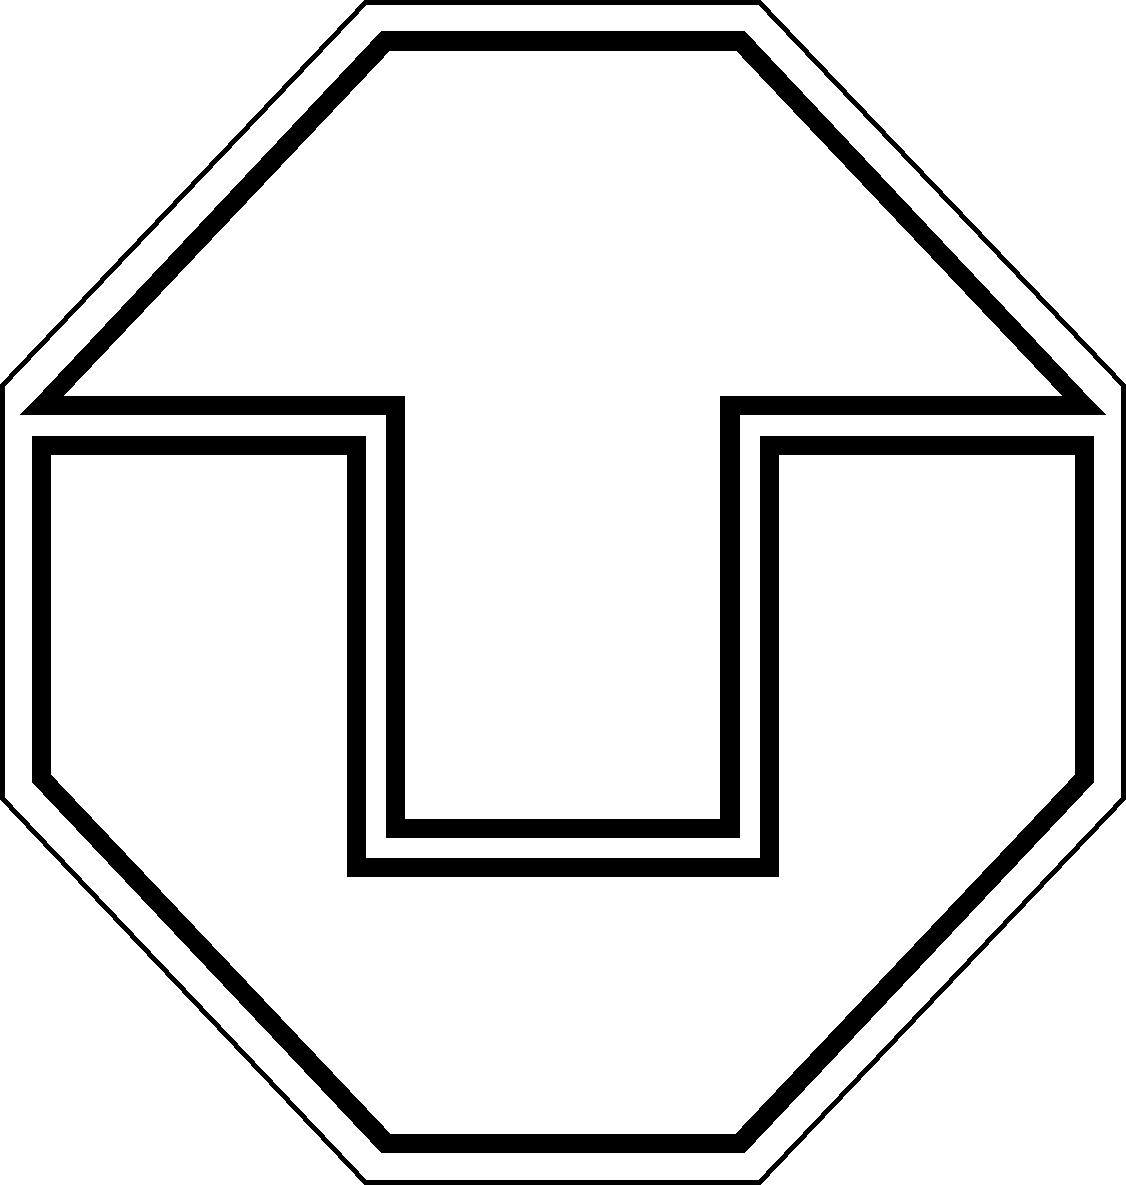
\includegraphics[width=3cm]{tu-logo}~\\[1cm]
\textsc{\LARGE Dresden University of Technology}\\[0.5cm]
\textsc{\Large Faculty of Computer Science}\\[0.2cm]
\textsc{\large Institute of Theoretical Computer Science}\\[0.2cm]
\textsc{\large Chair for Algebraic and Logical Foundations of Computer Science}\\[3cm]
\Huge Study's Thesis \\[1cm]
\huge Development and Analysis of Barrier Protocols\\[3cm]
\end{center}

\begin{flushleft} \large
	Author: Ronny Brendel \\
	Responsible university professor: Christel Baier \\
	Supervisors: Sascha Kl\"uppelholz \& Marcus V\"olp
\end{flushleft}

\vfill
\begin{flushright}
	\large October 2013
\end{flushright}

\end{titlepage}

\pagebreak
\newpage \thispagestyle{empty} \mbox{}
\pagebreak

%%%%%%%%%%%%%%%%%%%%%%%%%%%%%%%%%%%%%%%%%%%%%%%%%%%%%%%%%%%%%%%%%%%%%%%%%%%%%%%
\thispagestyle{empty}

%\section*{Aufgabenstellung}
%\label{sec:task}
%\begin{enumerate}
%	\item Literaturrecherche und ausf\"uhrlicher \"Uberblick aktuell genutzter Barrierenprotokolle sowie grunds\"atzlicher Implementierungsm\"oglichkeiten f\"ur Barrieren.
%	\item Untersuchung und Weiterentwicklung der von Nicolas Mc~Guire vorgeschlagenen Barriere.
%	\item Identifikation und Formalisierung der zentralen funktionalen Eigenschaften im Bezug auf Korrektheit sowie der quantitativen Eigenschaften zur Ermittlung der Performance von Barrierenprotokollen bez\"uglich Energieverbrauch und Geschwindigkeit.
%		\item Modellierung und Quantitative Analyse:
%			\begin{itemize}
%				\item Modellierung a) eines prominenten Vertreters von Barrierenprotokollen mit verteiltem Speicher, b) eines prominenten Vertreters von Barrierenprotokollen mit geteilten Speicher, c) des auf Mc~Guire beruhenden Barriereprotokolls jeweils im probabilistischem Model Checker PRISM.
%				\item Analyse und Vergleich der drei oben genannten Modelle im Bezug auf die in 3. identifizierten funktionalen sowie quantitativen Eigenschaften in PRISM. Wenn m\"oglich: Erg\"anzung des Performance-Vergleichs der drei Barrieren mittels messbasierter Methoden.
%			\end{itemize}
%		\item Zusammenfassung und Ausblick: Diskussion der in 4. gewonnenen Erkenntnisse
%\end{enumerate}
%
\section*{Task}
\label{sec:task}
\begin{enumerate}
	\item Literature research and detailed survey of currently used barrier protocols as well as implementation possibilities for barriers.
	\item Analysis and improvement of Nicolas Mc~Guire's proposed barrier.
	\item Identification and formalisation of key functional properties concerning correctness as well as quantitative aspects for determining performance of barrier protocols with regard to energy consumption and speed.
		\item Modelling and quantitative analysis:
			\begin{itemize}
				\item Modelling a) a prominent representative of barrier protocols for distributed memory, b) a prominent representative of barrier protocols for shared memory, c) the barrier protocol based on Mc~Guire's idea in each case using the probabilistic model checker PRISM.
				\item Analysis and comparison of the three above-mentioned models, regarding the functional as well as quantitative properties identified in 3., using PRISM. If possible: complement the performance evaluation of the three barriers using measurement-based methods.
			\end{itemize}
		\item Summary and outlook: Discussion of the insights gained in 4.
\end{enumerate}

\pagebreak
\newpage \thispagestyle{empty} \mbox{}
\pagebreak

%%%%%%%%%%%%%%%%%%%%%%%%%%%%%%%%%%%%%%%%%%%%%%%%%%%%%%%%%%%%%%%%%%%%%%%%%%%%%%%
\thispagestyle{empty}

%\section*{Selbstst\"andigkeitserkl\"arung}
%\label{sec:integrity}
%Ich erkl\"are hiermit, dass ich die vorliegende Arbeit selbst\"andig und ohne Benutzung anderer als der angegebenen Hilfsmittel angefertigt habe. Die aus fremden Quellen w\"ortlich oder sinngem\"a\ss ~\"ubernommenen Gedanken sind als solche kenntlich gemacht. Ich erkl\"are ferner, dass ich die vorliegende Arbeit an keiner anderen Stelle als Pr\"ufungsarbeit eingereicht habe oder einreichen werde.

\section*{Statement of academic integrity}
\label{sec:integrity}
I hereby declare that I prepared this thesis independently and without use of tools other than specified. Foreign thoughts, taken literally or in spirit, are marked as such. I also declare that I have not filed the present work at any other location or will submit it.

\pagebreak
\newpage \thispagestyle{empty} \mbox{}
\pagebreak

%%%%%%%%%%%%%%%%%%%%%%%%%%%%%%%%%%%%%%%%%%%%%%%%%%%%%%%%%%%%%%%%%%%%%%%%%%%%%%%
\thispagestyle{empty}

\renewcommand{\contentsname}{Table of contents}
\tableofcontents

\pagebreak
\newpage \thispagestyle{empty} \mbox{}
\pagebreak

%%%%%%%%%%%%%%%%%%%%%%%%%%%%%%%%%%%%%%%%%%%%%%%%%%%%%%%%%%%%%%%%%%%%%%%%%%%%%%%
\pagenumbering{arabic}
\section{Don't forget}
\begin{itemize}
	\item maybe add more $\sim$ into proper nouns to forbid separation
	\item present tense! Consistency please! Exception where it makes sense.
	\item maybe increase font size in charts
	\item "don't overuse passive voice"
	\item be very aware where you use thread and process, and make sure the reader understands when the distinction does not matter
	\item make clear what is meant in the listings
		\begin{itemize}
			\item C-esque pseudocode
			\item threadCount/processCount,  threadIndex/processIndex
			\item the code in the figures is executed on each thread. Each thread has an identifier between 0 and threadCount-1
			\item \& bit-wise \texttt{AND}, $|$ bit-wise \texttt{OR}, $\sim$ bit-wise \texttt{NOT}
			\item \texttt{x[$*$] := y} is short for assigning y to each element in x
			\item ?more?
		\end{itemize}
	\item mention that we assume atomic read and write at 32/64 bits a piece, when it matters
	\item explain cores vs processes, threads - we always assume threads, processes $>$= cores. Why. Find an appropriate spot to talk about this. I have marked a good spot in the text in Section~\ref{sssec:background-currently-used-shared}
	\item "be forthright about the limitations and assumptions of your design. Also, make sure you justify any shortcuts/limitations convincingly"
	\item \texttt{me} vs \texttt{threadIndex} / \texttt{processIndex}, make its use coherent
	\item color use in diagrams should be consistent (same bars should have same color across multiple diagrams)
	\item put raw data of figures into the appendix
\end{itemize}

%%%%%%%%%%%%%%%%%%%%%%%%%%%%%%%%%%%%%%%%%%%%%%%%%%%%%%%%%%%%%%%%%%%%%%%%%%%%%%%
\section{Introduction}
\label{sec:introduction}
\begin{itemize}
	\item \todo watch out that the intention/laying down a continuous thread is strong enough ((1)barriers can be improved, (2)through pW/CS, (3)model checking is useful)
	\item what is a barrier
	\item usage example for barriers
	\item barriers are common in parallel programming. OpenMP's\cite{openmp} implicit barriers. MPI barriers (Rolf Rabenseifner\cite{rab00}). Relate to normal send/recv, because absolute numbers without relation are not helpful.
		\begin{itemize}
			\item HLRS, year 2000
			\item many calls,
			\item 5.3\% of all time spent inside MPI calls, 0.7\% of all CPU time, estimated 1.6\% of the barrier execution time is actual synchronisation, 100\% minus 1.6\% is waiting for other processes to arrive, because of unbalanced computation. Average 1852 microsecond per call. (Figure~13 in paper)
			\item e.g. receive 12.9\% of all time spent inside MPI calls, 1.8\% of all cpu time, 33\% of the recv executation time is actual latency plus transfer time, 100\% minus 33\% is waiting for other processes to arrive, because of unbalanced comoputation. Average 498 microseconds per call.
		\end{itemize}
	\item motivation for researching barriers: Apply ideas of pW/CS\cite{pwcs} to other synchronisation primitives, e.g. barriers in order to gain performance, where performance can be any important measure e.g. speed, energy efficiency, (say something about possible improvements that can still be made).
	\item summarize pW/CS
		\begin{itemize}
			\item usually concurrent programs work in a deterministic fashion. That is the order and partners of remote synchronisation (locally, programs are obviously mostly deterministic) are predetermined. The algorithm is executed in a very controlled fashion. Same holds for synchronisation primitives themselves. Faulty behavior is avoided at great cost.
			\item don't avoid inconsistency at all cost. Make errors detectable, or ignorable.
			\item use the inherent randomness\cite{mcg09}, induced by caching, scheduling, randomness (ECC, flash access e.g.) at hardware level (jitter), or short: complexity of today's computer systems, in order to view concurrent accesses as really random. Thus we are able to apply probabilistic algorithms and analyse these algorithms using tools of probability theory.
			\item design algorithms that have sufficiently high probability of success and tolerate faulty behaviour.
			\item build them so that on average, or in their intended use case, they perform better than their deterministic counterparts, where better might e.g. be faster, more energy efficient, resource preserving.
			\item It seems to be a promising approach
			\item barriers can be improved. One possible way is through pW/CS.
		\end{itemize}
	\item how do we gather data on these algorithms to build confidence that they work properly, i.e. satisfy certain properties? And get a feeling for how they perform?
	\item Testing/Measurement (explain wording. Be aware of possible confusion) and model checking complement one another:
		\begin{itemize}
			\item Measurement is usually deterministic. If so, certain interesting states in a protocol are impossible to reach because of the randomness inherent to today's computers (add a short example? A special very case of a low level lock being contented?)
			\item Assuming you have randomized measurements, the probability to reach certain states in the protocol is so low that they are not revealed.
			\item Some parts of algorithms are performed in such a short time or need very exact preparation that it is practically impossible to analyse these parts using measurement. In this case model checking can be applied because it offers this granularity.
			\item Modelling has of course its own short comings. For example the state explosion problem.
			\item we can gain better quantitative insights into synchronisation protocols by combining both measurement and model checking.
		\end{itemize}
	\item briefly explain the report structure
		\begin{itemize}
			\item existing stuff
				\begin{itemize}
					\item means to implement barriers
					\item currently used barriers
					\item idea to split barriers into orthogonal parts and think about them separately
				\end{itemize}
			\item new barriers
			\item analysis and comparison of one old for shared memory and one old for distributed memory against the new barriers
			\item conclusion \& future work
		\end{itemize}
\end{itemize}

%%%%%%%%%%%%%%%%%%%%%%%%%%%%%%%%%%%%%%%%%%%%%%%%%%%%%%%%%%%%%%%%%%%%%%%%%%%%%%%
\section{Background}
\label{sec:background}
In this section we will first take look at the tools at our disposal to implement barriers on both shared memory and distributed memory architectures, followed by an overview of which barrier algorithms are used in today's parallel programming frameworks.
Finally we present a view of the barrier as a modularized algorithm consisting of various independent pieces.

%%%%%%%%%%%%%%%%%%%%%%%%%%%%%%%%%%%%%%%
\subsection{Means to implement barrier protocols}
\label{ssec:background-means}
A shared memory system consists of a number of processors which are connected to one chunk of memory. Information can be exchanged between processors by simply reading from and writing to the same memory location, since they all share the same address space.
Desktops, laptops and small to medium servers are typical examples of shared memory systems.

Many shared memory systems (called nodes) can be connected via a network to compose a distributed memory system. Such systems do not have one global memory, instead each of the nodes has its own private memory. Computation is done on each node using only local memory. In order to share information between nodes messages via network need to be exchanged.
For example large servers and high-performance computers are oftentimes distributed memory systems.

Programming for shared memory and distributed memory architectures is very different. Therefore we will subsequently differentiate between these two worlds.

%%%%%%%%%%%%%%%%%%%%
\subsubsection{Shared memory systems}
\label{sssec:background-means-shared}
A parallel program for a shared memory system consists of multiple threads of execution -- short \emph{threads}.

The straightforward way to share information between threads is to \emph{load} from and \emph{store} to the same memory address.

Furthermore most modern processors provide means to execute a small series of computations on a date while making the memory unavailable to other threads. They are called \emph{atomic operations}. Two examples are the \emph{test-and-set}- and \emph{add-fetch}-instruction. The former stores a value to an address if a given condition is fulfilled, the latter loads a date, adds a given value to it and stores it back.

Without these operations parallel programming is much more difficult and error-prone, since concurrently issuing normal load and store operations can easily cause \emph{race conditions}. This convenience, on the other hand, comes at the cost of additional management overhead for the processor. To date shared memory systems are usually limited to 64 threads and less. Some high-performance computing implementations reach numbers of 512 threads. In comparison distributed memory systems can have over a million processing units.

The intuitive ordering of concurrent memory accesses is \emph{sequentially consistent}.
\begin{quote}
	\textit{The result of any execution is the same as if the operations of all the processors were executed in some sequential order, and the operations of each individual processor appear in this sequence in the order specified by its program.} (Lamport~\cite{sequentialconsistency})
\end{quote}

Enforcing this intuitive semantic comes at a cost. Modern processors buffer memory operations on many levels. To enforce sequential consistency mechanisms to control and circumvent this buffering have to be introduced resulting in more transistors in the processor and higher memory access latency.

If an algorithm is carefully designed, one can weaken the consistency model to gain better performance. One prominent way of such a model is \textit{release consistency}~\cite{gha90}. Memory access appears unordered except for so called \emph{acquire} and \emph{release} operations. No memory access that has been issued after an acquire operation is permitted to finish before this acquire operation. No memory access is allowed to finish later than the next release operation. Acquire and release encapsulate the memory accesses in between.

Aside from implementing barriers in software vendors can wire a barrier implementation into the system's hardware. This is almost never done on shared memory architectures. One example for hardware barrier support is the SGI~UV~2000~\cite{sgiuv2000}, a high-performance shared memory computer.

%%%%%%%%%%%%%%%%%%%%
\subsubsection{Distributed memory systems}
\label{sssec:background-means-distributed}
A parallel program for a distributed memory architecture consists of multiple \emph{processes}. Each process has its own address space and is therefore unable to directly share memory with other processes.

First we will give an overview of general ways to implement synchronisation primitives on distributed memory systems followed by an analysis of one specific distributed memory programming standard.

One way to exchange information between two processes is via \emph{synchronous message passing}. Two processes meet at a point in time, exchange information, then part and continue their computational tasks. This method requires the involved peers to wait for each other, buffer and queue information and send it via network.

Another way to approach this is to wait as few as possible, since there is, for example, no need for a sending entity to wait until a receiver arrives. The sender might as well give his information to the communication framework and continue its computational work while the framework delivers the message as soon as the receiver is ready. This method is called \emph{asynchronous message passing}. Aside from less waiting time asynchronous message passing incurs similar overhead to synchronous message passing, because on the communication framework level the same work has to be done. The framework establishes network channels, buffers and queues data, and waits for the receiver to arrive.

A comparatively recent development is the move to \emph{remote memory access} (RMA). Remote memory access makes a portion of main memory available via network so that others can load from it and store to it without actively involving the memory's owning process. It is therefore sometimes called \emph{one-sided communication}. Implementations of RMA oftentimes support atomic operations.
In order for RMA to be available, the network hardware has to support it. For example InfiniBand~\cite{infiniband} has RMA facilities built in.
Due to its one-sided nature RMA incurs less overhead than the two previous techniques, but still buffers data. At very high networking bandwidths buffering data becomes a serious problem. To mitigate this vendors implement so called \emph{zero-copy} techniques.

Hardware support for barriers in distributed memory systems is widespread especially in high-performance computing. Examples include the Earth Simulator~\cite{earthsimulator}, IBM Blue Gene/L~\cite{bluegenel}, IBM Blue Gene/Q~\cite{bluegeneq} and a low-cost FPGA-based system~\cite{hoefler2006b}

Another interesting and seemingly untested approach is to use lossy communication channels for developing synchronisation protocols. Hardware is always erroneous. For example network packages conflict, packages drop, packages are corrupted or connections drop all the time. Reliability increasing techniques and protocols such as the Transmission Control Protocol (TCP), that are used to to mitigate these errors, incur a great performance penalty for transmitting short messages. TCP for example creates comparatively huge packages for small amounts of data, and each transmitted package has to be acknowledged by the receiver. Checking for flipped bits in the package adds further latency.
If one would instead craft algorithms so that they don't require 100\% reliable connections, further performance improvements are conceivable.
Two ways one could implement such algorithms are via the User Datagram Protocol (UDP)~\cite{udp} and InfiniBand's unreliable connections~\cite{infiniband}.

We will now investigate the facilities the Message Passing Interface (MPI)~\cite{mpi3}, the most prominent high-performance distributed programming interface, provides to implement barrier protocols. MPI is a standardised, low-level, language-independent and portable interface specification. It is very customizable and supports various modes of operation in order to support many different hardware configurations and allow the user to achieve maximum performance. MPI is widely adopted in high-performance computing and scientific computing\cite{mpiadoptiona, mpiadoptionb, mpiadoptionc} and there exist a variety of implementations in all major programming languages.

In our analysis we will only scratch the surface of what the standard offers, since diving deep involves lots of details, complicated semantics and many of the details don't matter for our purpose.

MPI supports synchronous message passing via \emph{send} and \emph{receive}. Additionally you can issue a send operation that immediately returns if no receiver is already in place waiting for the sender.

Furthermore MPI facilitates asynchronous message passing. One can send and receive messages without blocking and one can test if a message has been successfully transmitted. Synchronous and asynchronous message passing can be mixed. That means one is able to, for example, issue a non-blocking send that is matched by a blocking receive operation.

Since version 3.0 the MPI standard supports \emph{non-blocking collectives}. ``Collectives'' is a collective name for all communication operations where there is a variable number of communicating  peers, like barrier, broadcast, reduce and more.
Non-blocking collectives allow, in the example of the barrier, to not block at the operation but to register at the barrier upon arrival, and subsequently test the barrier for completion while doing computational work meanwhile.
This facility is probably unsuited for building new barriers on top of it, but is nevertheless an interesting recent development.

MPI also supports RMA. Although some MPI implementations, for example Open~MPI~\cite{openmpi}, do not yet support version 3.0 of the specification, we will restrict ourselves to analysing it, because it subsumes the features of version 2.2, it is already a year old and supported by other prominent implementations such as MPICH~3.0~\cite{mpich} and its derivatives MVAPICH2~\cite{mvapich} and Cray MPT~\cite{craympt}.

The definition of RMA according to the standard is rather involved, and we have to go into more detail to highlight important points.

To initiate sharing remote memory each participating process issues a collective call to create a \emph{window} of memory to be shared. A window is associated with the group of processes that created it, and through it each participating process exposes a portion of local memory to the other peers.
Upon creating a window a number of restrictions regarding the use of the window can be established in order to gain better performance. One can for example lower the memory consistency requirements or guarantee to not use certain operations.

Depending on the underlying hardware and MPI implementation there are two different memory models. A window may either have the \emph{separate} or the \emph{unified} model. The separate model states that the memory that is visible to the peers and the memory that is visible to the local process is not the same and might therefore not automatically update between these two copies. That means a change by a peer to one process's memory might not be made visible. This process has to manually update its local copy in order to see the change. In contrast the unified model makes sure that the two copies are eventually updated. Therefore manual refreshing is unnecessary. This differentiation is a direct result of trying to support many different hardware configurations.

Before going into the details of window synchronisation we have to introduce the concept of \emph{epochs}. An epoch is a period between two window synchronisation calls. RMA operations like \emph{put}, \emph{get}, \emph{accumulate} may only be used inside an epoch. Epochs are used to accumulate multiple operations to one larger transfer in order to achieve better efficiency.

MPI differentiates between \emph{active} and \emph{passive} target communication. In active target communication all peers are actively involved in window synchronisation, whereas in passive target communication only one side's activity is required.

One way to synchronise a window is via the \emph{fence} operation. A fence is a collective operation among all window group members that makes sure all outstanding RMA requests on this window are finished before the operation returns. It implies a full barrier synchronisation.

A more fine-grained instance of active target communication is via the operations \emph{start}, \emph{complete}, \emph{post} and \emph{wait}. Before issuing any remote access calls the issuing process first has to advertise his intention through the start operation. Once he is finished he will invoke the complete operation to announce that his transmission is complete. The receiving end similarly issues post and wait to expose and synchronise its memory. It is allowed to access his window's local memory meanwhile. In contrast to a fence operation one can restrict such synchronisation to arbitrary processes of the window.

The \emph{lock} and \emph{unlock} operations facilitate one way of passive target communication. Through these two functions one can block all access to a chunk of remote memory for all other window members. Between lock and unlock the process can then issue remote memory access operations without being interfered.

Another method to synchronise memory passively is through \emph{flush}. A flush makes sure all outstanding RMA calls, issued by the caller, are completed before returning. One can choose if the operations have to be completed only at the issuer's side or on the receiver's side as well.

Window synchronisation can be optimized through giving the implementation information about which operations are not used during the epoch and what happens before and after this synchronisation.

Inside an epoch one may issue remote memory access operations. The two simple ones are \emph{put} and \emph{get}. Memory access through put and get appears unordered inside an epoch.
Furthermore one can use atomic operations like \emph{accumulate}, \emph{fetch-and-op} or \emph{compare-and-swap}, with the intuitive semantic and where \emph{op} is a placeholder for various operations. The default global visibility order of atomic operations is sequentially consistent. When creating a window one can weaken this by, for example, allowing remote write operations to overtake remote read operations. Any combination of overtaking between reads, writes or between equal operations can be allowed.

Remote memory access in MPI is subject to a number of restrictions:
\begin{itemize}
	\item The buffer supplied to a put call should not be written to until the operation is finished.
	\item The buffer supplied to a get call should not be accessed until the operation is finished.
	\item The outcome of concurrent remote memory access to the same location inside an epoch is undefined.
	\item The outcome of concurrent local and remote access to the same location inside an epoch is undefined.
	\item The outcome of a single process issuing multiple put operations to the same location inside an epoch is undefined.
\end{itemize}
Therefore the only way to make sure that data is correctly written or read is through atomic operations or isolating access to the same location with costly window synchronisation operations.
Normally a processor commits 32 or 64 bit to main memory atomically, and in the remainder of this thesis we will assume this is the case.
Therefore these restrictions make sense for buffers at sizes above this, because concurrent memory access of interfering operations might overlap and the outcome is then indeed undefined.
For amounts of memory below this threshold we wish to have a semantic that is more specific. For example if two puts of at most 64 bits are concurrently issued to the same location, the outcome is that of the last put committed. Since this is not the case, MPI's restrictive RMA semantic makes it unsuitable to implement barrier algorithms, based on pW/CS's non-determinism ideas, on top of it.

Shared memory barriers usually rely on atomic operations. Most distributed memory barriers use synchronous message passing. These protocols have also been implemented using RMA to improve efficiency, but still behave equivalently.

%%%%%%%%%%%%%%%%%%%%%%%%%%%%%%%%%%%%%%%
\subsection{Currently used barrier protocols}
\label{ssec:background-currently-used}
Having surveyed the tools for implementing synchronisation primitives we will now examine the barrier protocols which power today's implementations for both shared and distributed memory systems.

%%%%%%%%%%%%%%%%%%%%
\subsubsection{Shared memory systems}
\label{sssec:background-currently-used-shared}

Many prominent implementations of shared memory concurrent programming facilities are part of closed source commercial products, like for example Intel Composer and Microsoft Visual Studio, and can therefore not be analysed. So we restrict ourselves to examining the GNU~C~Library~\cite{glibc} and GNU~OpenMP~\cite{gomp}.

% gnu-openmp/gcc-4.8.0/libgomp/libgomp.h, gnu-openmp/gcc-4.8.0/libgomp/barrier.c, gnu-openmp/gcc-4.8.0/libgomp/config/linux/, gnu-openmp/gcc-4.8.0/libgomp/config/linux/bar.h, gnu-openmp/gcc-4.8.0/libgomp/config/linux/bar.c, gnu-openmp/gcc-4.8.0/libgomp/config/linux/futex.h (cpu_relax), gnu-openmp/gcc-4.8.0/libgomp/config/linux/wait.h
The GNU~OpenMP implementation, included in the GNU Compiler Collection (GCC) version 4.8.0, implements a \emph{Central Counter Barrier}. Figure~\ref{fig:pseudocode-central-counter} describes the algorithm in pseudocode which is executed on each thread taking part in the barrier synchronisation.
The Central Counter Barrier uses the variable \texttt{barrier} to hold the number of threads that do not yet have arrived at the barrier. Initially it is assigned the number of threads. Upon entering the barrier each thread atomically decrements the variable by one and then waits until it reaches zero. After it reaches zero, all threads eventually leave the barrier.

\begin{figure}[H]
	\centering
	\begin{minipage}
\centering
\begin{lstlisting}[mathescape, linewidth=10.4cm]
shared variables: integer barrier := threadCount
$\listingrule{10.4cm}$

atomic{barrier := barrier - 1}

wait until barrier = 0
\end{lstlisting}
\end{minipage}

	\caption{Pseudocode of the Central Counter Barrier}
	\label{fig:pseudocode-central-counter}
\end{figure}

The protocol can be separated into two phases (Figure~\ref{fig:diagram-central-counter}). During the first phase each thread decrements the variable, and in the second reads the variable until it reaches the desired value.

\begin{figure}[H]
	\centering
	%\begin{tikzpicture}[node distance = 2.0cm, auto]
\begin{tikzpicture}[]

\node [draw=none]        (a)  {Atomic decrement:};
\node [o,   below of=a]  (0a) {0};
\node [o,   right of=0a] (1a) {1};
\node [o,   right of=1a] (2a) {2};
\node [o,   right of=2a] (3a) {3};
\node [o,   right of=3a] (4a) {4};
\node [box, below of=2a] (Va) {barrier};

\path [<->] (0a) edge (Va)
            (1a) edge (Va)
            (2a) edge (Va)
            (3a) edge (Va)
            (4a) edge (Va);

\node [draw=none, below of=0a]     (middle) {};

\node [draw=none, below of=middle] (b)      {Repeatedly read:};
\node [o,   below of=b]            (0b)     {0};
\node [o,   right of=0b]           (1b)     {1};
\node [o,   right of=1b]           (2b)     {2};
\node [o,   right of=2b]           (3b)     {3};
\node [o,   right of=3b]           (4b)     {4};
\node [box, below of=2b]           (Vb)     {barrier};

\path [->] (Vb) edge (0b)
           (Vb) edge (1b)
           (Vb) edge (2b)
           (Vb) edge (3b)
           (Vb) edge (4b);

\end{tikzpicture}

	\caption{Five threads performing the two phases of the Central Counter Barrier}
	\label{fig:diagram-central-counter}
\end{figure}

The actual implementation in GNU~OpenMP is more involved than the pseudocode in Figure~\ref{fig:pseudocode-central-counter} suggests. For example the algorithm shown here is destructive in the sense that it cannot be repeated, because if the variable is zero at the end, repetition would mean that the variable is negative in the next round, which breaks the protocol. To mitigate this the variable is copied, by each thread, upon first reading it and the last thread to enter resets the shared variable to its initial value.

The loop additionally keeps track number of unsuccessful reads. If this number reaches a certain amount, an operating system mechanism, called futex\cite{franke2002}, is employed to suspend the thread until a later time when the other threads hopefully have arrived. Through this back-off mechanism the system avoids unnecessary busy waiting which would negatively impact power consumption. The threshold of this counter is architecture specific and set to an equivalent of about 3 milliseconds of waiting on GNU/Linux. In case the number of threads is larger than the number of physical cores, i.e. the processor is oversubscribed, the counter is set to a much lower value. This way the operating system scheduler can switch between threads more quickly so that threads that need time for computation are not blocked by busy waiting ones.

Throughout this thesis we will assume that the thread and process count is at most as high as the number of physical processor cores in a system, because oversubscription is not useful inside a single program and therefore rarely happens.

% glibc/nptl/sysdeps/pthread/pthread.h, glibc/nptl/pthread_barrier_*, glibc/nptl/sysdeps/unix/sysv/linux/internaltypes.h
The GNU POSIX Threads implementation, called Native POSIX Threads Library (NPTL), is part of the The GNU~C~Library.
The basic barrier algorithm used in it is the same as for GNU~OpenMP. One main differences is that it does not use atomic operations to decrement the variable, but explicitly locks it to guard from interfering access. Second there is no busy waiting, but upon arriving at the barrier the thread will immediately suspend, via a futex, and wait to be woken up by the last thread arriving. The third difference is that to reset the barrier each thread atomically increments the barrier variable by one upon leaving.

%%%%%%%%%%%%%%%%%%%%
\subsubsection{Distributed memory systems}
\label{sssec:background-currently-used-distributed}

In this section we present the barrier algorithms that are used in the two major open source MPI implementations, namely Open~MPI~\cite{openmpi} and MPICH~\cite{mpich}. We restrict our analysis to MPI for the same reasons we only considered MPI in Section~\ref{sssec:background-means-distributed}.

% ompi/mca/coll/tuned/coll_tuned_barrier.c : ompi_coll_tuned_barrier_intra_recursivedoubling, ompi_coll_tuned_barrier_intra_bruck, ompi/mca/coll/tuned/coll_tuned_decision_fixed.c
Open~MPI distinguishes between process counts that are powers of two and which are not. If it is a power of two, a \emph{recursive doubling} barrier is used. A detailed explanation of this protocol can be found in \cite{hoefler2005}. For non-power-of-two process counts Open~MPI uses the \emph{Dissemination Barrier}, introduced by Hensgen, Finkel and Manber in 1988~\cite{hensgen1988}.

Figure~\ref{fig:pseudocode-dissemination} presents the pseudocode of this algorithm, which is executed on each process individually. A process is identified by its \emph{process index}, which is a number between 0 and $\mathit{processCount} - 1$. For readability reasons we have chosen an RMA-esque representation of the protocol, although it can similarly be implemented using message passing techniques.
In contrast to the Central Counter Barrier, the Dissemination Barrier uses not only one variable but an array of boolean variables per process involved. Each of these arrays is located in the local memory of its owning process and is initially set to false.
The protocol is organised in rounds. Each round the distance (variable \texttt{dist}) to the next two partners, to read from and write to, doubles. Process indices  are always calculated modulo the total number of processes to achieve a wraparound. Figure~\ref{fig:diagram-dissemination} illustrates this communication pattern.

\begin{figure}[htbp]
	\centering
	\begin{center}
\begin{minipage}{\textwidth}
\begin{lstlisting}[mathescape, linewidth=11.2cm]
constants:        me := processIndex
shared variables: boolean
                  barrier[processCount][processCount]
local variables:  integer dist, to, from
initialisation:   barrier[*][*] := false
$\listingrule{11.2cm}$

dist := 1
while dist < processCount {
	to   := (me + dist) (mod processCount)
	from := (me - dist) (mod processCount)
	
	barrier[to][me] := true
	
	wait until barrier[me][from] = true

	dist := dist $\cdot$ 2
}
\end{lstlisting}
\end{minipage}
\end{center}

	\caption{Pseudocode of the Dissemination Barrier}
	\label{fig:pseudocode-dissemination}
\end{figure}

\begin{figure}[htbp]
	\centering
	%\begin{tikzpicture}[node distance = 2.0cm, auto]
\begin{tikzpicture}[]

%pivotal nodes
\node [draw=none                 ]   (a) {Round 1:};
\node [o, below of=a             ]  (0a) {0};
\node [below of=0a, draw=none    ]   (b) {Round 2:};
\node [o, below of=b             ]  (0b) {0};
\node [below of=0b, draw=none    ]   (c) {Round 3:};
\node [o, below of=c             ]  (0c) {0};

\clip (-0.5cm,0) rectangle (7.5cm,-6cm);

% round 1
\node [   left of=0a , draw=none ] (07a);
\node [o, right of=0a            ]  (1a) {1};
\node [o, right of=1a            ]  (2a) {2};
\node [o, right of=2a            ]  (3a) {3};
\node [o, right of=3a            ]  (4a) {4};
\node [o, right of=4a            ]  (5a) {5};
\node [o, right of=5a            ]  (6a) {6};
\node [o, right of=6a            ]  (7a) {7};
\node [o, right of=7a, draw=none ] (70a);

\path [->] (07a) edge [distance=0.2cm]  (0a)
            (0a) edge [distance=0.2cm]  (1a)
            (1a) edge [distance=0.2cm]  (2a)
            (2a) edge [distance=0.2cm]  (3a)
            (3a) edge [distance=0.2cm]  (4a)
            (4a) edge [distance=0.2cm]  (5a)
            (5a) edge [distance=0.2cm]  (6a)
            (6a) edge [distance=0.2cm]  (7a);
\path [-]   (7a) edge [distance=0.2cm] (70a);

% round 2
\node [   left of=0b , draw=none ] (07b);
\node [   left of=07b, draw=none ] (06b);
\node [o, right of=0b            ]  (1b) {1};
\node [o, right of=1b            ]  (2b) {2};
\node [o, right of=2b            ]  (3b) {3};
\node [o, right of=3b            ]  (4b) {4};
\node [o, right of=4b            ]  (5b) {5};
\node [o, right of=5b            ]  (6b) {6};
\node [o, right of=6b            ]  (7b) {7};
\node [o, right of=7b, draw=none ] (70b);
\node [o, right of=70b, draw=none] (71b);

\path [->] (06b) edge [distance=0.6cm]                 (0b)
           (07b) edge [distance=0.6cm,out=-45,in=225]  (1b)
            (0b) edge [distance=0.6cm]                 (2b)
            (1b) edge [distance=0.6cm,out=-45,in=225]  (3b)
            (2b) edge [distance=0.6cm]                 (4b)
            (3b) edge [distance=0.6cm,out=-45,in=225]  (5b)
            (4b) edge [distance=0.6cm]                 (6b)
            (5b) edge [distance=0.6cm,out=-45,in=225]  (7b);
\path [-]   (6b) edge [distance=0.6cm]                (70b)
            (7b) edge [distance=0.6cm,out=-45,in=225] (71b);

%round 3
\node [   left of=0c , draw=none ] (07c);
\node [   left of=07c, draw=none ] (06c);
\node [   left of=06c, draw=none ] (05c);
\node [   left of=05c, draw=none ] (04c);
\node [o, right of=0c            ]  (1c) {1};
\node [o, right of=1c            ]  (2c) {2};
\node [o, right of=2c            ]  (3c) {3};
\node [o, right of=3c            ]  (4c) {4};
\node [o, right of=4c            ]  (5c) {5};
\node [o, right of=5c            ]  (6c) {6};
\node [o, right of=6c            ]  (7c) {7};
\node [   right of=7c , draw=none] (70c);
\node [   right of=70c, draw=none] (71c);
\node [   right of=71c, draw=none] (72c);
\node [   right of=72c, draw=none] (73c);

\path [->] (04c) edge [distance=0.8cm]  (0c)
           (05c) edge [distance=0.8cm,out=-45,in=225]  (1c)
           (06c) edge [distance=0.8cm]  (2c)
           (07c) edge [distance=0.8cm,out=-45,in=225]  (3c)
            (0c) edge [distance=0.8cm]  (4c)
            (1c) edge [distance=0.8cm,out=-45,in=225]  (5c)
            (2c) edge [distance=0.8cm]  (6c)
            (3c) edge [distance=0.8cm,out=-45,in=225]  (7c);
\path [-]   (4c) edge [distance=0.8cm] (70c)
            (5c) edge [distance=0.8cm,out=-45,in=225] (71c)
            (6c) edge [distance=0.8cm] (72c)
            (7c) edge [distance=0.8cm,out=-45,in=225] (73c);

\end{tikzpicture}

	\caption{The rounds of the Dissemination Barrier}
	\label{fig:diagram-dissemination}
\end{figure}

At first a process notifies the next one that is has arrived at the barrier by setting the array element at index \texttt{me} on the next process to true. Then it waits until the previous one notifies its arrival. When that happens the waiting process enters the next round. It now knows that itself, and the previous process have arrived at the barrier and notifies the process at double the previous distance (2) of its knowledge by setting its array element at the target process to true. Through this communication pattern the number of processes, that each process knows have arrived, doubles with each round. Thus after $\lceil \log_2 \mathit{processCount} \rceil$ rounds every process knows of the arrival of all others and can therefore leave the barrier.

Notifying the next process is done via writing to remote memory, and waiting for notification via busy waiting on local memory. The number of remote access operations per round is the same as the number of processes involved.

The actual implementation in Open~MPI uses MPI's \emph{send-receive} operation instead of our version's remote write and local read. This operation sends a message and waits for another at the same time. The protocol is not destructive because send and receive do not change the state of the protocol. Therefore no resetting mechanism, as used by GNU~OpenMP for the Central Counter Barrier, is needed.
Open~MPI is able to replace this implementation with hardware specific ones, if it detects supported hardware. For example InfiniBand uses a variation of the Dissemination Barrier based on RMA\cite{hoefler2006a}.

% src/mpi/coll/barrier.c : MPIR_Barrier_intra
MPICH version 3.0, which forms the basis of many other prominent MPI implementations like MVAPICH2 and Cray~MPT, implements the same send-receive-based Dissemination Barrier as is used in Open~MPI, but disregards the number of processes.

Aside from distributed memory architectures it is possible to implement these protocols for shared memory systems, as has been demonstrated for the Intel~XEON~Phi~\cite{hoefler2013}.

%%%%%%%%%%%%%%%%%%%%%%%%%%%%%%%%%%%%%%%
\subsection{Barrier building blocks}
\label{ssec:background-building-blocks}
During our analysis of general implementation facilities and concrete barrier implementations we observed that one can assemble barriers from orthogonal components.

One independent piece is the employed way of reinitializing the barrier after use. As we have seen for the Central Counter Barrier (Section~\ref{sssec:background-currently-used-shared}) resetting might be achievable through slight modification of the algorithm. This does not work for all protocols, though.

Another possibility is to replace boolean variables, as used in the Dissemination Barrier in Figure~\ref{fig:pseudocode-dissemination}, with a repetition counter. The remote write and local spin-waiting condition are then replaced with atomic increment and a test for the correct number of repetitions. The additional amount of memory needed is linear in the number of processes. The added computational overhead is negligible.

A way of resetting that works in all circumstances is to use three distinct barriers and switch cleverly between them. The proposed procedure, to be executed by each process individually, is illustrated in Figure~\ref{fig:pseudocode-triple-reset}. In the beginning the first two barriers are initialized, whereas the third one is set to the state of a finished barrier. Upon entering the routine one uses the barrier which comes after the currently finished barrier and resets the one which has been finished before. This approach is provably correct, uses triple the amount of memory of a single barrier, and ads minimal computational overhead.

\begin{figure}[htpb]
	\centering
	\begin{center}
\begin{minipage}{\textwidth}
\begin{lstlisting}[mathescape, linewidth=9.3cm]
shared state:   barrier1, barrier2, barrier3
initialization: barrier1 := initialized
                barrier2 := initialized
                barrier3 := finished
$\listingrule{9.3cm}$

if barrier3 is finished {
	use barrier1
	reset barrier3
} else if barrier1 is finished {
	use barrier2
	reset barrier1
} else if barrier2 is finished {
	use barrier3
	reset barrier2
}
\end{lstlisting}
\end{minipage}
\end{center}

	\caption{Pseudocode of the triple barrier reset approach}
	\label{fig:pseudocode-triple-reset}
\end{figure}

In order to lower power consumption limiting the amount of busy waiting is important for barrier implementations. Choosing a back-off strategy can be done independently of the used barrier protocol. In almost all cases one wants to take apart the waiting loop and insert a suspension mechanism.

During the first initialisation of the barrier an implementation can decide how to handle the case where the number of threads or processes exceeds the number of physical processor cores. Therefore implementing a solution to this scenario is orthogonal to the other algorithm components.

Another useful approach is to assemble multiple different barrier protocols to create a new one. For example assume you have a hardware topology of shared memory nodes which are connected via network. It is conceivable to construct a barrier that executes a Central Counter Barrier on each node, and then one process of each node takes part in a Dissemination Barrier. After the Dissemination Barrier is completed the intra-node processes are notified and the assembled barrier completes.
This way one can reap the benefits of the best performing barrier on each level of the topology.
This might also make sense if barrier algorithms vary in performance for different numbers of threads or processes.

%%%%%%%%%%%%%%%%%%%%%%%%%%%%%%%%%%%%%%%%%%%%%%%%%%%%%%%%%%%%%%%%%%%%%%%%%%%%%%%
\section{New barriers}
\label{sec:new}
In this section we first present a new variation on a barrier protocol of ours. The second algorithm reverses the approach of the Central Counter Barrier. Third we demonstrate a pW/CS-influenced modification of the second barrier.

%%%%%%%%%%%%%%%%%%%%%%%%%%%%%%%%%%%%%%%
\subsection{MGB Barrier}
\label{ssec:new-mgb}
The original idea of the following algorithm is part of a private communique between Nicholas Mc~Guire, the pW/CS-inventor, and us. Figure~\ref{fig:pseudocode-mgb} presents the new barrier, which is a variation of the protocol first mentioned in \cite{bre13}. It is intended for shared memory architectures.

\begin{figure}[htbp]
	\centering
	\begin{center}
\begin{minipage}{\textwidth}
\begin{lstlisting}[mathescape, linewidth=11.6cm]
constants:        me:=$2^\mathit{threadIndex}$, full:=$\sum_{i=0}^{\mathit{threadCount}-1}2^i$
local variables:  integer copy
shared variables: integer first, second, current
initialisation:   first := 0, second := 0, current := 1
$\listingrule{11.6cm}$

if current = 1 {

	do {
		copy := (copy $\&$ $\sim$me) | first
		if copy $\&$ me = 0 {
			copy  := copy | me
			first := copy
		}
	} while copy $\neq$ full and current = 1

	current := 2
	second  := 0

} else if current = 2 {

	do {
		copy := (copy $\&$ $\sim$me) | second
		if copy $\&$ me = 0 {
			copy := copy | me
			second := copy
		}
	} while copy $\neq$ full and current = 2

	current := 1
	first   := 0
}
\end{lstlisting}
\end{minipage}
\end{center}

	\caption{Pseudocode of the MGB Barrier}
	\label{fig:pseudocode-mgb}
\end{figure}

Before going into detail, we first have to repeat some of the notation used in the pseudocode. It borrows from the C programming language. \&, $|$ and $\sim$ are the bitwise \emph{and}, \emph{or} and \emph{not} operator. The constant \texttt{threadIndex} is a thread identifying number between 0 and $\mathit{threadCount}-1$.

The protocol consists of two symmetric sub-barriers. It uses \texttt{current}, a variable which holds the number of the sub-barrier that is currently used, to switch between them.
Through \texttt{first} and \texttt{second} the barrier keeps track of which threads have arrived.
The variable \texttt{copy} is a local copy of either \texttt{first} or \texttt{second}.
A thread commits itself to \texttt{first} or \texttt{second} by setting its respective bit to 1. In the pseudocode we implement this bit set behaviour through integers and working with powers of two. If all threads committed themselves to one of the sub-barriers, it is a full bit set equal to the constant \texttt{full}.
All threads participating in the barrier synchronisation enter the same of the two parts.
Inside a loop participants try to synchronise. When successful the barrier is reset through the two subsequent assignments of \texttt{current} and either \texttt{first} or \texttt{second}.

Initially \texttt{first} and \texttt{second} are zero, and \texttt{current} is one. When a thread arrives at the barrier it will enter the upper if-branch. It then asks which threads have already arrived, adds himself to the acquired bit set, and stores it back to the variable \texttt{first}.
He then repeatedly polls \texttt{first} in order to find out if his commitment attempt has been overwritten, i.e. its bit is not set anymore, by another thread's concurrently issued write operation, and secondly to determine whether the barrier is completed. The upper barrier is completed, if either \texttt{first} equals \texttt{full} or \texttt{current} is 2. The first thread to realise that \texttt{first} has been set to \texttt{full} will exit the loop, set \texttt{current} to 2 and continue his computational work. Subsequently all other threads eventually leave the barrier.
When entered again the same procedure is executed in the lower if-branch using the variable \texttt{second} instead of \texttt{first}. A third repetition utilises the upper branch again.

The presented protocol reflects the ideas of pW/CS in that it loosely organizes communication between threads and is less enforcing in the sense that threads may overwrite each others' commitment attempts.

In comparison to the Central Counter Barrier this approach does not rely on the existence atomic operations.

The number of threads this protocol supports is limited by the number of bits a processor can atomically commit, which is usually 64 bits. To alleviate this problem one can implement an array-based variant of the protocol. Instead of reading \texttt{first} and \texttt{second} one copies the array element by element. Comparing is \texttt{done} element by element as well. Instead of setting the variable one writes back only the one element where the thread's bit resides on. This way writing still requires only one atomic 64-bit commitment.

%%%%%%%%%%%%%%%%%%%%%%%%%%%%%%%%%%%%%%%
\subsection{B1 Barrier}
\label{ssec:new-b1}

The following barrier protocol reverses the idea of the Central Counter Barrier (Section~\ref{sssec:background-currently-used-shared}) to use a single global counter that all threads atomically access once and read repeatedly. Instead it uses an array of boolean variables, one element for each thread, which is also accessed differently.
The algorithm's pseudocode, executed individually on each thread taking part, is depicted in Figure~\ref{fig:pseudocode-b1}.

\begin{figure}[htbp]
	\centering
	\begin{center}
\begin{minipage}{\textwidth}
\begin{lstlisting}[mathescape, linewidth=9.7cm]
shared variables: boolean barrier[threadCount]
local variables:  integer i
initialization:   barrier[*] := false
$\listingrule{9.7cm}$

barrier[threadIndex] := true

i := 0
while i < threadCount {
	if barrier[i] = false {
		i := -1
	}
	i = i + 1
}
\end{lstlisting}
\end{minipage}
\end{center}

	\caption{Pseudocode of the B1 Barrier}
	\label{fig:pseudocode-b1}
\end{figure}

Initially each array element is false. Upon arriving at the barrier a thread registers itself by setting its array element to true. He subsequently queries all other threads for arrival. As soon as it finds one that has not yet arrived, it resets the loop counter and begins querying all others anew. Once all threads arrive, eventually each of them will leave, thus completing the barrier synchronisation.

Similar to the Central Counter Barrier the protocol can be split into two phases (Figure~\ref{fig:diagram-central-counter}).
The two differences are that, because each thread writes only to its own array element, they don't require atomic access to register themselves at the barrier, and during the reading phase each thread has to read each other thread's variable instead of polling just a single global one. The threads may concurrently write, but have to spend more time reading.

The Barrier cannot be repeated as is. A way to add resetting to the protocol is by using the repetition counter approach introduced in Section~\ref{ssec:background-building-blocks}. In order to avoid false~sharing~\cite{falsesharing}, which would majorly degrade performance, an actual implementation of the protocol allocates one cache line for each array element. Cache lines are usually 64 bytes large. Therefore transforming the array into an array of counters does not require more memory.

A small improvement to the shown algorithm is to keep track of the first few threads that have successfully arrived. The loop counter is then reset to this number instead of 0.

Since we don't use any central information, this protocol can be implemented for both shared and distributed memory architectures.

%%%%%%%%%%%%%%%%%%%%%%%%%%%%%%%%%%%%%%%
\subsection{B2 Barrier}
\label{ssec:new-b2}
The B2 Barrier is a variation on the previous barrier in which less communication is traded for more computation.

In principle the following protocol can be implemented on both shared and distributed memory architectures. We now switch to a distributed setting, because preliminary analysis showed that the saved memory access cost in comparison to the additional computational overhead favours its use in a distributed scenario.

Figure~\ref{fig:pseudocode-b2} presents the B2 Barrier's RMA-style pseudocode. The notation used in this listing is explained in Section~\ref{ssec:new-mgb}.

\begin{figure}[htbp]
	\centering
	\begin{center}
\begin{minipage}{\textwidth}
\begin{lstlisting}[mathescape, linewidth=10.7cm]
constants:        me := processIndex, meBit := $2^{me}$,
                  full := $\sum_{i=0}^{\mathit{processCount}-1}2^i$
shared variables: integer barrier[processCount]
local variables:  integer i
initialization:   barrier[*] := 0
                  i := processIndex
$\listingrule{10.7cm}$

barrier[me] := meBit;

do {
	do {
		i := i + 1 (mod processCount)
	} while barrier[me] $\&$ $2^i$ = 1

	barrier[me] := barrier[me] | barrier[i]
} while barrier[me] $\neq$ full
\end{lstlisting}
\end{minipage}
\end{center}

	\caption{Pseudocode of the B2 Barrier}
	\label{fig:pseudocode-b2}
\end{figure}

Each array element of \texttt{barrier} is located in the local memory of the process with the matching index. These elements are bit sets representing the knowledge of the owning process about the arrival of others.

When the first process arrives at the barrier it registers itself by setting its bit in its local array element and then continues to query the remote processes. It only acquires a remote array element, if it did not yet successfully do so, i.e. the remote process's bit is not set in the local bit set. If this is the case, it fetches the remote element and adds it to its own, thus adding the arrival of all processes the remote end knows about to its own bit set. Querying the other processes is repeated until the bit set indicates that all processes arrived.

Comparing this behaviour to the B1 Barrier, a process now locally keeps track of the processes that have arrived and only queries those where the owning process did not yet get an affirmative answer.
The protocol does not maintain the differentiation between reading and writing phase since it keeps updating its local variable during the loop.

This protocol writes only locally, and reads only remotely. It does not rely on the existence of atomic operations.

In comparison to other distributed memory barrier protocols, e.g. the Dissemination Barrier (Section~\ref{sssec:background-currently-used-distributed}), the communication pattern is largely random. The order of remote access depends on remote memory access latency, local computation and memory access speed, the exact time of arrival of each process and operating system influences like scheduling. The effect of these factors combined makes the order of communication practically random.

Like the B1 Barrier this protocol is destructive. One can add resetting via the triple barrier method presented in Section~\ref{ssec:background-building-blocks}.

Like the MGB Barrier this protocol is restricted to 64 processes. An extension to arrays of bit sets can be implemented in the same way as described in Section~\ref{ssec:new-mgb}.

%%%%%%%%%%%%%%%%%%%%%%%%%%%%%%%%%%%%%%%%%%%%%%%%%%%%%%%%%%%%%%%%%%%%%%%%%%%%%%%
\section{Analysis and comparison}
\label{sec:analysis}
% maybe distinguish extreme cases vs more normal cases. And the spectrum in between -- adds structure -- is nice.

In this section we will evaluate one commonly used barrier for each shared and distributed memory architectures. In both categories we compare the chosen protocol to one of our newly presented ones.

Early evaluations have shown the MGB Barrier to perform worse than the Central Counter Barrier, whereas the B1 and B2 Barrier show promise. Therefore we restrict our attention to these two.

In the shared memory setting the Central Counter Barrier is pitted against the B1 Barrier. In the distributed memory case we compare the Dissemination to the B2 Barrier.

In our evaluation we assume no back-off strategy is used. This means if a variable is repeatedly requested inside a loop, it is fetched as often as program execution speed allows. The topic of back-off strategies is a subject in its own right and goes beyond the scope of this thesis.

The analysis is split into two parts. First we present properties, perceivable without measurement and modelling, that are inherent to the protocols. Second we employ model checking to quantify our observations and gain a deeper understanding of the chosen barriers.

%%%%%%%%%%%%%%%%%%%%%%%%%%%%%%%%%%%%%%%
\subsection{General properties}
\label{sssec:analysis-general}
This section is divided into two parts: shared and distributed memory barriers.
In each we present the memory requirement of the algorithms.
For the Central Counter and B1 Barrier we additionally consider properties of the reading and writing phase.
In the distributed memory scenario we are also interested in the remote access behaviour of both chosen protocols.

%%%%%%%%%%%%%%%%%%%%
\paragraph{Shared memory barriers}
\label{sssec:analysis-general-shared}
% - don't talk cache specifics, because we have not given an introduction to MSI. Express yourself in simple terms.
% - make sure that people understand it is about shared read/write, not local variables.

The Central Counter Barrier (Figure~\ref{fig:pseudocode-central-counter} in Section~\ref{sssec:background-currently-used-shared}) and the B1 Barrier (Figure~\ref{fig:pseudocode-b1} in Section~\ref{ssec:new-b1}) are both divided into two phases: the reading and the writing phase.

In the writing phase of the Central Counter Barrier concurrently issued add-fetch operations are serialised, because atomic operations on a single variable cannot be executed in parallel. On the other hand the B1 Barrier allocates one array element per thread. Therefore all write operations can be performed concurrently. If all threads arrive in the same instant, the commitment of all threads takes only as long as one write operation does, therefore speeding up this process by a factor of $n$, where $n$ is the number of threads participating. In a more balanced scenario, i.e. processes arrive in intervals, this advantage over the Central Counter Barrier diminishes.

During the reading phase of the Central Counter Barrier a thread fetches a single variable repeatedly until it has the desired value. A thread in the B1 Barrier needs to read between 1 and $n$ array elements before it can leave the loop.

The B1 Barrier has the edge in the writing phase, whereas the Central Counter Barrier performs well during reading. We attempt to quantify the effect of this behaviour in Section~\ref{ssec:analysis-modelchecking}.

The memory required by the Central Counter Barrier is logarithmic in the number of threads. With a 64-bit counter up to $2^{64}$ threads can be synchronised. The B1 Barrier uses a linear amount of memory -- $\mathit{threadCount} \cdot 64$ bytes, assuming a cache line is 64 bytes large. This might seem like a lot, but since shared memory systems rarely exceed 512 cores, a maximum of only 32 KiB is used.

%%%%%%%%%%%%%%%%%%%%
\paragraph{Distributed memory barriers}
\label{sssec:analysis-general-distributed}
In this section we assume $n$ to be the number of processes participating in the barrier synchronisation.

The Dissemination Barrier (Figure~\ref{fig:pseudocode-dissemination} and \ref{fig:diagram-dissemination} in Section~\ref{sssec:background-currently-used-distributed}) and the B2 Barrier (Figure~\ref{fig:pseudocode-b2} in Section~\ref{ssec:new-b2}) communicate very differently.

The minimum number of remote access operations required to perform a barrier synchronisation is $2 \cdot (n-1)$. Figure~\ref{fig:diagram-gather-broadcast} illustrates a simple gather and broadcast  barrier (process zero gathers all arrival notifications and broadcasts to all processes when the barrier is complete) using this number of operations. It does so in $2 \cdot  \lceil \log _2~n \rceil$ rounds. All operations inside a round can be executed in parallel. However rounds themselves are completed serially. In order to lower the number of rounds to $\lceil \log _2~n \rceil$ the Dissemination Barrier issues $n \cdot \lceil \log _2~n \rceil$, more than the minimum needed, remote access operations. The added communication overhead is traded for a decrease in overall execution time.

\begin{figure}[htbp]
	\centering
	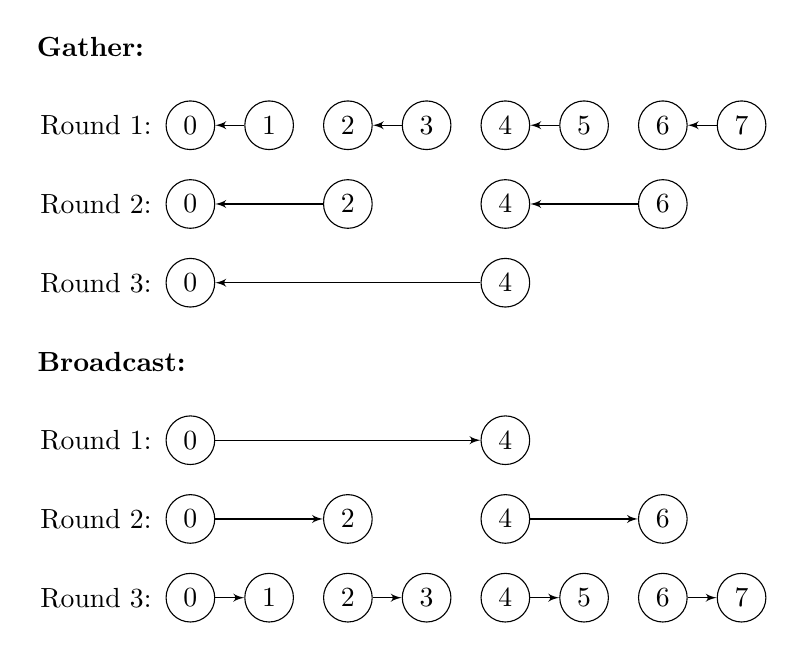
\begin{tikzpicture}[]

%pivotal nodes
\node [               draw=none  ]   (a) {};
\node [left of=a     ,draw=none,distance=2cm  ]  (ya) {\textbf{Gather:~~~~~}};
\node [o, below of=a,            ]  (0a) {0};
\node [o, below of=0a            ]  (0b) {0};
\node [o, below of=0b            ]  (0c) {0};
\node [below of=0c   , draw=none ]   (d) {};
\node [left of=d     , draw=none ]  (yd) {\textbf{Broadcast:}};
\node [o, below of=d             ]  (0d) {0};
\node [o, below of=0d            ]  (0e) {0};
\node [o, below of=0e            ]  (0f) {0};

% gather 1
\path (0a) ++(180:1.2cm) node []    (xa) {Round 1:};
\node [o, right of=0a            ]  (1a) {1};
\node [o, right of=1a            ]  (2a) {2};
\node [o, right of=2a            ]  (3a) {3};
\node [o, right of=3a            ]  (4a) {4};
\node [o, right of=4a            ]  (5a) {5};
\node [o, right of=5a            ]  (6a) {6};
\node [o, right of=6a            ]  (7a) {7};

\path [<-] (0a) edge (1a)
           (2a) edge (3a)
           (4a) edge (5a)
           (6a) edge (7a);

% gather 2
\path (0b) ++(180:1.2cm) node []    (xb) {Round 2:};
\node [o, right of=0b,draw=none  ]  (1b) {};
\node [o, right of=1b            ]  (2b) {2};
\node [o, right of=2b,draw=none  ]  (3b) {};
\node [o, right of=3b            ]  (4b) {4};
\node [o, right of=4b,draw=none  ]  (5b) {};
\node [o, right of=5b            ]  (6b) {6};
\node [o, right of=6b,draw=none  ]  (7b) {};

\path [<-] (0b) edge (2b)
           (4b) edge (6b);

% gather 3
\path (0c) ++(180:1.2cm) node []    (xc) {Round 3:};
\node [o, right of=0c,draw=none  ]  (1c) {};
\node [o, right of=1c,draw=none  ]  (2c) {};
\node [o, right of=2c,draw=none  ]  (3c) {};
\node [o, right of=3c            ]  (4c) {4};
\node [o, right of=4c,draw=none  ]  (5c) {};
\node [o, right of=5c,draw=none  ]  (6c) {};
\node [o, right of=6c,draw=none  ]  (7c) {};

\path [<-] (0c) edge (4c);

% broadcast 1
\path (0d) ++(180:1.2cm) node []    (xd) {Round 1:};
\node [o, right of=0d,draw=none  ]  (1d) {};
\node [o, right of=1d,draw=none  ]  (2d) {};
\node [o, right of=2d,draw=none  ]  (3d) {};
\node [o, right of=3d            ]  (4d) {4};
\node [o, right of=4d,draw=none  ]  (5d) {};
\node [o, right of=5d,draw=none  ]  (6d) {};
\node [o, right of=6d,draw=none  ]  (7d) {};

\path [->] (0d) edge (4d);

% broadcast 2
\path (0e) ++(180:1.2cm) node []    (xe) {Round 2:};
\node [o, right of=0e,draw=none  ]  (1e) {};
\node [o, right of=1e            ]  (2e) {2};
\node [o, right of=2e,draw=none  ]  (3e) {};
\node [o, right of=3e            ]  (4e) {4};
\node [o, right of=4e,draw=none  ]  (5e) {};
\node [o, right of=5e            ]  (6e) {6};
\node [o, right of=6e,draw=none  ]  (7e) {};

\path [->] (0e) edge (2e)
           (4e) edge (6e);

% broadcast 3
\path (0f) ++(180:1.2cm) node []    (xf) {Round 3:};
\node [o, right of=0f            ]  (1f) {1};
\node [o, right of=1f            ]  (2f) {2};
\node [o, right of=2f            ]  (3f) {3};
\node [o, right of=3f            ]  (4f) {4};
\node [o, right of=4f            ]  (5f) {5};
\node [o, right of=5f            ]  (6f) {6};
\node [o, right of=6f            ]  (7f) {7};

\path [->] (0f) edge (1f)
           (2f) edge (3f)
           (4f) edge (5f)
           (6f) edge (7f);

\end{tikzpicture}

	\caption{Communication pattern of the gather and broadcast barrier}
	\label{fig:diagram-gather-broadcast}
\end{figure}

Because of its random communication pattern there is no fixed number of remote accesses issued by the B2 Barrier. The number of successful, non-zero, remote reads, lies between $2 \cdot (n-1)$ and $n \cdot (n-1)$. The amount of unsuccessful reads is not limited, since the loop remotely polls other processes until all arrive.

Where a process in the Dissemination Barrier waits for one designated communication partner each round, the B2 Barrier does not wait for a single process but instead continues to poll the next one.

Requiring $\lceil \log _2~n \rceil$ rounds is obviously worse than $\log _2~n$. Especially from $n$, where $n$ is a power of two, to $n+1$ processes the number of rounds increases by 1. Therefore the runtime is expected to show a stair-esque behaviour. Every time the number of rounds increases the duration of the barrier increases by a large step, whereas adding more processes to the same number of rounds adds little overhead.
In contrast to this the execution time of the B2 Barrier is distributed evenly.

Synchronisation using the Dissemination and B2 Barrier requires the same amount of memory. In principle $\lceil \log _2~n \rceil$ bits per process suffice for both algorithms. The Dissemination variant shown in Figure~\ref{fig:pseudocode-dissemination} uses a total of $n^2$ bits, but, since each process receives from only $\lceil \log _2~n \rceil$ other processes, a modified array index calculation would allow the protocol to work with $n \cdot \lceil \log _2 ~n \rceil$ bits.

Assuming all processes arrive at a similar time, Figure~\ref{fig:diagram-dissemination} in Section~\ref{sssec:background-currently-used-distributed} illustrates the progression through the rounds of the Dissemination Barrier. More often than not, processes arrive in large intervals, compared to the execution time of a barrier itself.
Therefore some processes advance through the rounds before every process arrived.
But how far exactly can the protocol progress without all processes?

Suppose every process but the fourth has entered the barrier. Figure~\ref{fig:diagram-dissemination-progress} then shows the advance of the processes through the rounds.

\begin{figure}[htbp]
	\centering
	%\begin{tikzpicture}[node distance = 2.0cm, auto]
\begin{tikzpicture}[]

%pivotal nodes
\node [o, below of=xxx]  (0a) {0};
\path (0a) ++(-90:1.4cm) node [draw, circle, node] (0b) {0};
\path (0b) ++(-90:1.8cm) node [draw, circle, node] (0c) {0};

\path (0a) ++(180:1.4cm) node [node] (xa) {Round 1:};
\path (0b) ++(180:1.4cm) node [node] (xb) {Round 2:};
\path (0c) ++(180:1.4cm) node [node] (xc) {Round 3:};

\clip (-0.5cm,0) rectangle (7.5cm,-6cm);

% round 1
\node [   left of=0a , draw=none ] (07a) {};
\node [o, right of=0a            ]  (1a) {1};
\node [o, right of=1a            ]  (2a) {2};
\node [o, right of=2a            ]  (3a) {3};
\node [o, right of=3a, dotted    ]  (4a) {4};
\node [o, right of=4a            ]  (5a) {5};
\node [o, right of=5a            ]  (6a) {6};
\node [o, right of=6a            ]  (7a) {7};
\node [o, right of=7a, draw=none ] (70a) {};

\path [->] (07a) edge [distance=0.2cm        ]  (0a)
            (0a) edge [distance=0.2cm        ]  (1a)
            (1a) edge [distance=0.2cm        ]  (2a)
            (2a) edge [distance=0.2cm        ]  (3a)
            (3a) edge [distance=0.2cm        ]  (4a)
            (4a) edge [distance=0.2cm, dotted]  (5a)
            (5a) edge [distance=0.2cm        ]  (6a)
            (6a) edge [distance=0.2cm        ]  (7a);
\path [-]   (7a) edge [distance=0.2cm        ] (70a);

% round 2
\node [   left of=0b , draw=none ] (07b) {};
\node [   left of=07b, draw=none ] (06b) {};
\node [o, right of=0b            ]  (1b) {1};
\node [o, right of=1b            ]  (2b) {2};
\node [o, right of=2b            ]  (3b) {3};
\node [o, right of=3b, dotted    ]  (4b) {4};
\node [o, right of=4b, dotted    ]  (5b) {5};
\node [o, right of=5b            ]  (6b) {6};
\node [o, right of=6b            ]  (7b) {7};
\node [o, right of=7b, draw=none ] (70b) {};
\node [o, right of=70b, draw=none] (71b) {};

\path [->] (06b) edge [distance=0.6cm                       ]  (0b)
           (07b) edge [distance=0.6cm,out=-45,in=225        ]  (1b)
            (0b) edge [distance=0.6cm                       ]  (2b)
            (1b) edge [distance=0.6cm,out=-45,in=225        ]  (3b)
            (2b) edge [distance=0.6cm                       ]  (4b)
            (3b) edge [distance=0.6cm,out=-45,in=225        ]  (5b)
            (4b) edge [distance=0.6cm               , dotted]  (6b)
            (5b) edge [distance=0.6cm,out=-45,in=225, dotted]  (7b);
\path [-]   (6b) edge [distance=0.6cm                       ] (70b)
            (7b) edge [distance=0.6cm,out=-45,in=225        ] (71b);

%round 3
\node [   left of=0c , draw=none ] (07c) {};
\node [   left of=07c, draw=none ] (06c) {};
\node [   left of=06c, draw=none ] (05c) {};
\node [   left of=05c, draw=none ] (04c) {};
\node [o, right of=0c            ]  (1c) {1};
\node [o, right of=1c            ]  (2c) {2};
\node [o, right of=2c            ]  (3c) {3};
\node [o, right of=3c, dotted    ]  (4c) {4};
\node [o, right of=4c, dotted    ]  (5c) {5};
\node [o, right of=5c, dotted    ]  (6c) {6};
\node [o, right of=6c, dotted    ]  (7c) {7};
\node [   right of=7c , draw=none] (70c) {};
\node [   right of=70c, draw=none] (71c) {};
\node [   right of=71c, draw=none] (72c) {};
\node [   right of=72c, draw=none] (73c) {};

\path [->] (04c) edge [distance=0.8cm               , dotted]  (0c)
           (05c) edge [distance=0.8cm,out=-45,in=225, dotted]  (1c)
           (06c) edge [distance=0.8cm               , dotted]  (2c)
           (07c) edge [distance=0.8cm,out=-45,in=225, dotted]  (3c)
            (0c) edge [distance=0.8cm                       ]  (4c)
            (1c) edge [distance=0.8cm,out=-45,in=225        ]  (5c)
            (2c) edge [distance=0.8cm                       ]  (6c)
            (3c) edge [distance=0.8cm,out=-45,in=225        ]  (7c);
\path [-]   (4c) edge [distance=0.8cm               , dotted] (70c)
            (5c) edge [distance=0.8cm,out=-45,in=225, dotted] (71c)
            (6c) edge [distance=0.8cm               , dotted] (72c)
            (7c) edge [distance=0.8cm,out=-45,in=225, dotted] (73c);

\end{tikzpicture}

	\caption{Progression through the rounds of the Dissemination Barrier with process four not having entered}
	\label{fig:diagram-dissemination-progress}
\end{figure}

Every dotted line indicates a remote write operation that does not happen. Processes with dotted circles have not reached the current round.
Since process four does not notify process five of its arrival, in the second round process four and five do not advertise their arrival to process six and zero. The number of stuck processes doubles each round.
Once process four enters, the missing remote operations in all three rounds are still to be completed until the processes may leave the barrier.

Table~\ref{tab:table-dissemination-progress} illustrates which process knows of which other's arrival through the rounds of the Dissemination Barrier and for the B2 Barrier. The formula below each subtable title indicates the number of processes that are known to have arrived.

\begin{table}[htbp]
\centering
\caption{Which process knows of which other's arrival}
\vspace{0.2cm}
\begin{minipage}{0.42\linewidth}
	\textbf{Diss. after round 1:} \\
	$(n-1) + (n-1) = 14$ \\
	\vspace{-0.1cm} \\
	\resizebox{5cm}{!}{
		\begin{tabular}{c | c c c c c c c c}
			  & 0        & 1        & 2        & 3        & 4 & 5        & 6        & 7 \\
			\hline
			0 & $\times$ &          &          &          &         &          &          & $\times$ \\
			1 & $\times$ & $\times$ &          &          &         &          &          &          \\
			2 &          & $\times$ & $\times$ &          &         &          &          &          \\
			3 &          &          & $\times$ & $\times$ &         &          &          &          \\
			4 &          &          &          & $\times$ &         &          &          &          \\
			5 &          &          &          &          &         & $\times$ &          &          \\
			6 &          &          &          &          &         & $\times$ & $\times$ &          \\
			7 &          &          &          &          &         &          & $\times$ & $\times$ \\
		\end{tabular}
	}
\end{minipage}
\begin{minipage}{0.42\linewidth}
	\textbf{Diss. after round 2:} \\
	$14 + 6 \cdot 2 = 26$ \\
	\vspace{-0.1cm} \\
	\resizebox{5cm}{!}{
		\begin{tabular}{c | c c c c c c c c}
			  & 0        & 1        & 2        & 3        & 4 & 5        & 6        & 7 \\
			\hline
			0 & $\times$ &          &          &          &   & $\times$ & $\times$ & $\times$ \\
			1 & $\times$ & $\times$ &          &          &   &          & $\times$ & $\times$ \\
			2 & $\times$ & $\times$ & $\times$ &          &   &          &          & $\times$ \\
			3 & $\times$ & $\times$ & $\times$ & $\times$ &   &          &          &          \\
			4 &          & $\times$ & $\times$ & $\times$ &   &          &          &          \\
			5 &          &          & $\times$ & $\times$ &   & $\times$ &          &          \\
			6 &          &          &          &          &   & $\times$ & $\times$ &          \\
			7 &          &          &          &          &   &          & $\times$ & $\times$ \\
		\end{tabular}
	}
\end{minipage}
\begin{minipage}{0.42\linewidth}
	\vspace{0.3cm}
	\textbf{Diss. after round 3}: \\
	$26 + 4 \cdot 4 = 44$ \\
	\vspace{-0.1cm} \\
	\resizebox{5cm}{!}{
		\begin{tabular}{c | c c c c c c c c}
			  & 0        & 1        & 2        & 3        & 4 & 5        & 6        & 7 \\
			\hline
			0 & $\times$ &          &          &          &        & $\times$ & $\times$ & $\times$ \\
			1 & $\times$ & $\times$ &          &          &        &          & $\times$ & $\times$ \\
			2 & $\times$ & $\times$ & $\times$ &          &        &          &          & $\times$ \\
			3 & $\times$ & $\times$ & $\times$ & $\times$ &        &          &          &          \\
			4 & $\times$ & $\times$ & $\times$ & $\times$ &        & $\times$ & $\times$ & $\times$ \\
			5 & $\times$ & $\times$ & $\times$ & $\times$ &        & $\times$ & $\times$ & $\times$ \\
			6 & $\times$ & $\times$ & $\times$ &          &        & $\times$ & $\times$ & $\times$ \\
			7 & $\times$ & $\times$ & $\times$ & $\times$ &        &          & $\times$ & $\times$ \\
		\end{tabular}
	}
\end{minipage}
\begin{minipage}{0.42\linewidth}
	\vspace{0.3cm}
	\textbf{B2 Barrier:} \\
	$(n-1) \cdot (n-1) = 49$ \\
	\vspace{-0.1cm} \\
	\resizebox{5cm}{!}{
		\begin{tabular}{c | c c c c c c c c}
			  & 0        & 1        & 2        & 3        & 4 & 5        & 6        & 7 \\
			\hline
			0 & $\times$ & $\times$ & $\times$ & $\times$ &   & $\times$ & $\times$ & $\times$ \\
			1 & $\times$ & $\times$ & $\times$ & $\times$ &   & $\times$ & $\times$ & $\times$ \\
			2 & $\times$ & $\times$ & $\times$ & $\times$ &   & $\times$ & $\times$ & $\times$ \\
			3 & $\times$ & $\times$ & $\times$ & $\times$ &   & $\times$ & $\times$ & $\times$ \\
			4 &          &          &          &          &   &          &          &          \\
			5 & $\times$ & $\times$ & $\times$ & $\times$ &   & $\times$ & $\times$ & $\times$ \\
			6 & $\times$ & $\times$ & $\times$ & $\times$ &   & $\times$ & $\times$ & $\times$ \\
			7 & $\times$ & $\times$ & $\times$ & $\times$ &   & $\times$ & $\times$ & $\times$ \\
		\end{tabular}
	}
\end{minipage}
\label{tab:table-dissemination-progress}
\end{table}

Because the number of blocked processes doubles each round the ratio of stuck to not-stuck processes is worse for non-power-of-two than it is for power of two process counts.

The B2 Barrier does not work in rounds and does not have designated communication partners. It therefore fetches all other process's arrival notifications while one is missing.

When the last process arrives the Dissemination Barrier requires at least as many serial remote writes as there are rounds, whereas the B2 Barrier issues its remaining remote reads concurrently. The number of remaining remote access operations is $2^{\lceil \log_2~n \rceil} - 1$ for the Dissemination Barrier and $n$ for the B2 Barrier.

We attempt to quantify the influence of this behaviour on the execution time and energy consumption in the following section.

%%%%%%%%%%%%%%%%%%%%%%%%%%%%%%%%%%%%%%%
\subsection{Model checking}
\label{ssec:analysis-modelchecking}
The properties, we are interested in, can be divided into two broad categories: functional and quantitative properties. Functional properties describe the supposed behaviour of the barriers, whereas quantitative properties express conditions that rely on probabilistic aspects of the protocols, e.g. execution time.

To check correctness of the barriers we model every instance where execution is random through non-deterministic choice. This yields a Markov decision process (MDP), which we then use a basis for automated analysis with the SPIN model checker.

To model the inherent randomness of our algorithms we use exponential distributions. This way we obtain continuous-time Markov chains (CTMCs) which serve a basis for formal quantitative analysis using the PRISM model checker.

Models are obtained in a compositional way, using action labels and global state to synchronise.

%%%%%%%%%%%%%%%%%%%%
\subsubsection{Preliminaries}
\label{sssec:analysis-modelchecking-preliminaries}
In this section we repeat principles of continuous-time Markov chains that are of interest to our analysis. Further details can be found in textbooks on Markov chains, e.g. \cite{kul95, ks76}. Some of this Section borrows from \cite{bai13}

If $S$ is a finite set, then a distribution on $S$ is a function $\nu:S \rightarrow [0,1]$ with $\sum\limits_{s \in S} \nu (s) = 1$.

A CTMC $\mathcal{M}$ is a tuple $(S, \mathit{Act}, R, \mu)$ where $S$ is a finite set of states, $Act$ a finite set of action names and $R$ a function of type $S \times \mathit{Act} \times S \rightarrow \mathbb{R}_{\ge 0}$, called the rate matrix of $\mathcal{M}$. $\mu$ is a distribution on $S$ specifying the probabilities for the initial states.

If $R(s, \alpha, s') = \lambda$ (short $s \xrightarrow{\lambda : \alpha} s'$) and $\lambda > 0$ then $\mathcal{M}$ has a transition from $s$ to $s'$ with action label $\alpha$ and rate $\lambda$.
$\lambda$ specifies the rate of the exponential distribution. That means the probability for the transition $s \xrightarrow{\lambda : \alpha} s'$ to be ready for firing some time in the interval $[0,t]$ is $1-e^{- \lambda t}$. The average delay of this transition is $\frac{1}{\lambda}$.
If $R(s, \alpha, s') = 0$ then there is no transition in $\mathcal{M}$ from $s$ to $s'$ via $\alpha$.
The choice between multiple enabled transitions is made by the following condition.
The probability to trigger a particular transition $s \xrightarrow{\lambda : \alpha} s'$ is $P(s, \alpha, s') = \frac{\lambda}{E(s)}$ where $E(s)$ is the exit rate of state $s$, i.e. the sum of the rates of all outgoing transitions of state $s$.
The probability that $s \xrightarrow{\lambda : \alpha} s'$ will fire within $t$ time units is then $P(s, \alpha, s') \cdot (1 - e^{- E(s) \cdot t})$.

Paths in a CTMC are sequences of consecutive transitions augmented by the time points when they are taken.
We employ the logic CSL~\cite{assb96, bhhk00, knp07} to analyse such transition systems.
To specify sets of infinite paths, we will use an LTL-like notation, such as $\lozenge T$ (``eventually T'') and $\square T$ (``always T'') where $T$ is a set of states.
Instead of naming states we will oftentimes use state predicates, combined using propositional formulas, to describe sets of states. Their meaning will be obvious from the context.

We will also study reward based properties formalized using the logic CSRL~\cite{bhhk00, knp07}.
This requires the extension of $\mathcal{M}$ by two reward functions. The state reward function $\mathit{srew} : S \rightarrow \mathbb{R}$ specifies the reward earned per time unit while being in state $s$. The transition reward function $\mathit{trew} : S \times S \rightarrow \mathbb{R}$ assigns a reward to each transition between two states regardless of action labels.
For finite paths one can then reason about accumulated reward and reachability reward.
Suppose $\pi$ is a finite path where the underlying state sequence is $s_1 s_2 ...s_n$ and let $t_0 = 0$ and $t_i$ the time point where $\pi$ takes the $i$-th transition.
The accumulated reward of $\pi$ is then
\begin{center}
	$\mathit{Rew}(\pi) = \mathlarger{\sum}\limits_{i=0}^{n-1} \big( (t_{i+1} - t_i) \cdot \mathit{srew}(s_i) + \mathit{trew}(s_i, s_{i+1}) \big)$
\end{center}
It is the sum, over all states but the last, of the state rewards multiplied by the time spent in each state plus the reward assigned to each transition between consecutive states in $\pi$.
The reachability reward is defined as
\begin{center}
	$\mathrm{ReaRew}(\pi, \Phi) = \mathit{Rew}(\pi(s_0:s_j))$
\end{center}
where $j = min \{ i~|~s_i \models \Phi \}$ and  $\pi(s_0:s_j)$ stands for the sub-path of $\pi$ starting in $s_0$ and ending in $s_j$.
The extension of these notions from paths to states and CTMCs is done the usual way and can be found in \cite{bhhk03}

Analysing the protocols we will for example deal with the state reward function that assigns value 1 to each state. In this case $\mathrm{ReaRew}(\Phi)$ can be interpreted as the average number of processor clock cycles to reach a state where $\Phi$ holds.
We also wish to count remote memory access operations. For this we assign value 1 to each transition that represents such an operation. $\mathrm{ReaRew}(\Phi)$ is then the average number of remote memory access operations issued until reaching a $\Phi$-state.

%%%%%%%%%%%%%%%%%%%%
\subsubsection{Modelling}
\label{sssec:analysis-modelchecking-modelling}
To analyse functional and quantitative aspects of the chosen barrier protocols, we model them using two different formalisms and two different software tools. We use ordinary non-stochastic transition systems and the SPIN~\cite{spin, hol97} model checker to verify functional properties. To analyse quantitative properties we employ CTMCs and PRISM~\cite{prism, knp09}.

To verify the functional correctness of a barrier, we need to include a reset mechanism into the model, which is not needed for quantitative analysis. By stripping this unnecessary information off the probabilistic model we shrink its state space. This enables us to verify properties more quickly and/or on larger models.

Depending on circumstances we describe part of a system as non-stochastic control flow diagram and part as CTMC. Control flow diagrams contain local variables, shared variables, control flow information and need to be unwound to form a proper CTMC. The state space of the resulting CTMC is then a combination of control flow location and variable assignments.

The CTMCs of the protocols are composed of multiple modules.
Composed modules are executed in an interleaved fashion except if transitions require synchronising actions. A synchronising action is an action that can be triggered by at least two modules. A transition with such an action can only fire if all modules, that are able to fire this action eventually, are presently in a state where a transition with this action label is enabled. The rate of such a simultaneous transition is determined by any one module. For each simultaneous transition, in our case, only one module specifies a rate.
The presented way of composing modules corresponds to the following SOS rules.

If no other module uses action label $\alpha$:
\begin{center}
	$\mathlarger{\frac{s \xrightarrow{\lambda : \alpha} s'}{\langle s , \overline{x} \rangle \xrightarrow{\lambda : \alpha} \langle s', \overline{x} \rangle}}$
\end{center}
where $\overline{x}$ is the tuple of local state of all other modules. The module's execution is interleaved with that of all other modules.
If $\alpha$ is used by two modules:
\begin{center}
	$\mathlarger{\frac{s \xrightarrow{\lambda : \alpha} s', t \xrightarrow{\alpha} t'}{\langle s, t , \overline{x} \rangle \xrightarrow{\lambda : \alpha} \langle s', t', \overline{x} \rangle}}$
\end{center}
Only if $\alpha$ is enabled in both modules, these two transitions fire simultaneously.

Analogous rules apply for more than two modules sharing an action label.

%%%%%%%%%%
\paragraph{Shared memory}
\label{sssec:analysis-modelchecking-modelling-shared-memory}
In order to exchange information threads write to and read from the same memory location.
Memory access latency is very large in comparison to the duration of arithmetic operations.
Because synchronisation is mainly about exchanging information between threads, the execution time of barrier protocols is dominated by memory access latency.

Usually memory access is cached. That means repeatedly reading a value is quick, because upon first reading it the processor places a copy of it near its execution units. When a cached value gets changed by another thread that shares it, the cached value needs to be thrown away because otherwise it would soon be incoherent.
In order to model execution time and energy consumption of a barrier protocol, we therefore model the caching behaviour of threads.

We identify a shared variable with the cache line it resides on. A cache line is usually a 64 bytes large unit of contiguous memory to which all cache manipulation operations are applied as a whole. It increases the granularity of address space, which is usually one byte, to decrease management overhead for caching.
Each thread that has access to this shared variable has one copy of such a cache line.
Synchronisation between cache line copies and with other CTMC modules, like the actual algorithm to be modelled, is done via synchronising actions. The operation triggering thread's cache line copy determines the rate of the transition.
For convenience we use combinations of action labels like $\alpha \lor \beta$ meaning that there are two transitions, one with action $\alpha$ and one with $\beta$ between two states. Either action may trigger the transition.

We use the MSI cache coherency protocol, extended by support for atomic operations, to model cache consistency. The MSI protocol is a basic cache model. Further details about it can be found online at for example~\cite{msi}.

In the MSI model a cache line copy can be in one of three states. \emph{Modified} means the thread has the only up-to-date copy of the cache line and all other copies are \emph{invalid}. If a cache line copy is invalid it is outdated and therefore not usable. Being in the \emph{shared} state means the thread has an up-to-date copy, but other threads may have a correct copy, too. We extend these three states by a fourth, called \emph{atomic}. Its meaning is the same as modified, except that as long as a cache line copy is in this state, no other thread may access it.

Figure~\ref{fig:model-shared-memory} illustrates how a cache line copy changes its state. Solid transitions are fired by events occurring on the thread owning the cache line copy, whereas dashed transitions are due to events triggered by other cache line copies.

\begin{figure}[htbp]
	\centering
	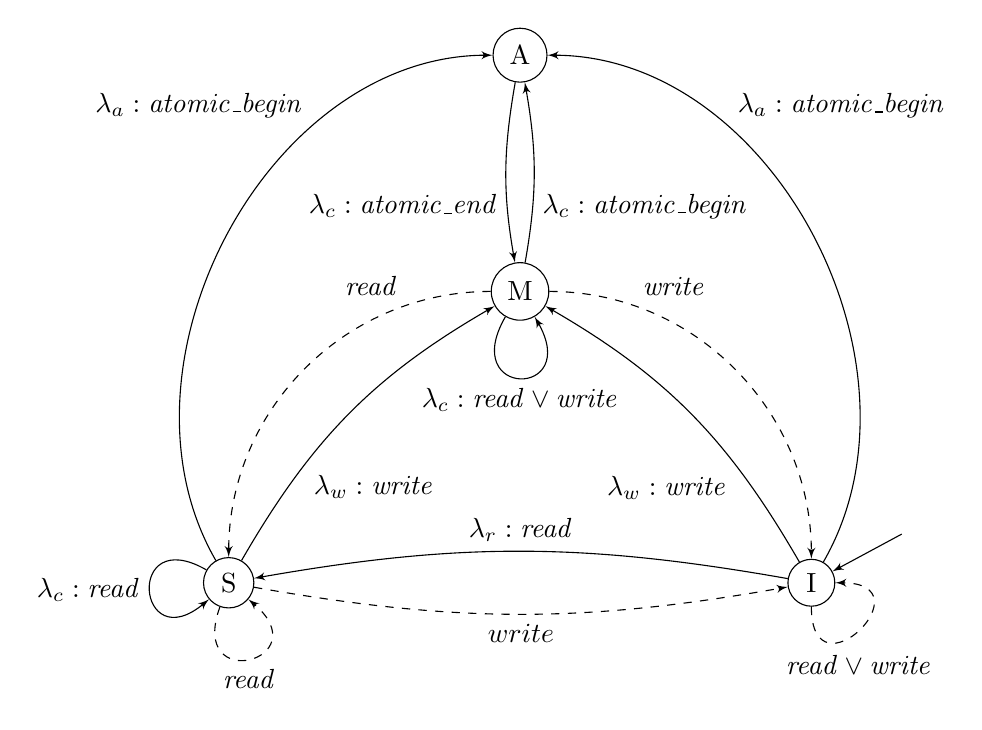
\begin{tikzpicture}[]

% nodes
\node [o]            at (  0  ,  3   ) (A)    {A};
\node [o]            at (  0  ,  0   ) (M)    {M};
\node [o]            at ( -3.7, -3.7 ) (S)    {S};
\node [o]            at (  3.7, -3.7 ) (I)    {I};
\node [o, draw=none] at (  5.0, -3.0 ) (init) {};

%  edges
\path [->]
  (init) edge                                                 node []                     {}                                     (I)

  (A)    edge [in=100, out=260]                               node [left       , pos=0.7] {$\lambda_c : \mathit{atomic\_end}$}   (M)

  (M)    edge [in=-80, out=80]                                node [right      , pos=0.3] {$\lambda_c: \mathit{atomic\_begin}$}  (A)
  (M)    edge [loop, distance=1.2cm, in=-60, out=240]         node [below] {$\lambda_c: \mathit{read} \lor \mathit{write}$}      (M)
  (M)    edge [dashed, in=90, out=180]                        node [above left , pos=0.2] {$\mathit{read}$}                      (S)
  (M)    edge [dashed, in=90, out=0]                          node [above right, pos=0.2] {$\mathit{write}$}                     (I)

  (S)    edge [in=180, out=120]                               node [above left , pos=0.7] {$\lambda_a : \mathit{atomic\_begin}$} (A)
  (S)    edge [in=210, out=60]                                node [below right, pos=0.3] {$\lambda_w : \mathit{write}$}         (M)
  (S)    edge [loop, distance=1.2cm, in=220, out=150]         node [left]                 {$\lambda_c : \mathit{read}$}          (S)
  (S)    edge [loop, dashed, distance=1.2cm, in=320, out=250] node [below]                {$\mathit{read}$}                      (S)
  (S)    edge [dashed, in=190, out=-10]                       node [below]                {$write$}                              (I)

  (I)    edge [in=0, out=60]                                  node [above right,pos=0.7]  {$\lambda_a : \mathit{atomic\_begin}$} (A)
  (I)    edge [in=-30, out=120]                               node [below left ,pos=0.3]  {$\lambda_w : \mathit{write}$}         (M)
  (I)    edge [in=10, out=170]                                node [above]                {$\lambda_r : \mathit{read}$}          (S)
  (I)    edge [loop, dashed, distance=1.2cm, in=0, out=-90]   node [below=0.2cm]          {$\mathit{read} \lor \mathit{write}$}  (I);

\end{tikzpicture}

	\caption{CTMC of a shared memory variable}
	\label{fig:model-shared-memory}
\end{figure}

For example if a thread reads a variable and its own cache line copy is invalid, it first needs to make sure that all other threads take notice and change its cache line copy state to shared in case it was modified before. After this the thread fetches the cache line from main memory, marks its own copy shared, reads the variable and continues program execution.

The durations of the cache line copy state transitions are as follows.
Reading a modified or shared copy is considered instantaneous, because the copy is up-to-date and no other copies need to be notified.
If a thread whose copy is invalid reads a variable, it has to advertise its intent to all other copies. If another copy is modified, it needs to switch to the shared state. Meanwhile the reading thread fetches an up-to-date copy from main memory, sets the state of its local copy to shared, and finally continues program execution. This usually takes around 50 processor clock cycles.
A write operation on a modified variable is considered instantaneous, since no other thread has an up-to-date copy and therefore no one needs to be notified.
If the cache line copy in question is shared or invalid, it broadcasts an invalidation request to all other copies, and waits until every copy fulfills the request. After this the thread can safely mark his copy modified and finally write to it. This operation commonly takes about 100 cycles.
Entering the atomic state works exactly like entering the modified state.
During the atomic state the cache line copy postpones all requests to this copy until it transitions to a different state. After leaving the atomic state, it instantly begins to answer these requests. Therefore leaving the atomic state is considered instantaneous.

The exact number of processor clock cycles these operations take is strongly hardware-dependent. For the CTMC model we assume a cache read to take 50 cycles, whereas writing and entering an atomic operation requires 100 cycles. The rates of the transitions corresponding to the described events is then the reciprocal of the cycle count.
The rate of an instantaneous operation, which is assumed to be one cycle, is $\lambda_c = 1$. The rate of a cache read is $\lambda_r = \frac{1}{50}$. And the rate of initiating a write or an atomic operation is $\lambda_w = \lambda_a = \frac{1}{100}$

For technical reasons we switch the rate of entering and leaving an atomic operation. The intuitive result is the same.

%%%%%%%%%%
\paragraph{Central Counter Barrier}
\label{sssec:analysis-modelchecking-modelling-central-counter}
The Central Counter Barrier uses one shared variable. Therefore the final CTMC is composed of one cache line copy module per thread and one algorithm module per thread.
The algorithm's control flow diagram (Figure~\ref{fig:model-central-counter}) directly results from the pseudocode in Figure~\ref{fig:pseudocode-central-counter} (Section~\ref{sssec:background-currently-used-shared}).

\begin{figure}[htbp]
	\centering
	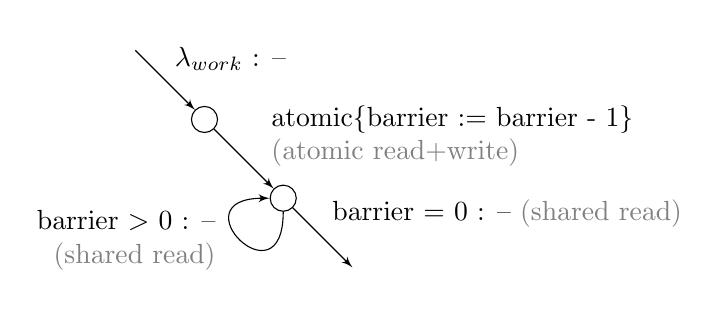
\begin{tikzpicture}[node distance = 2.0cm, auto]

% nodes
\node [o, draw=none] at ( 0 ,  0 ) (init) {};
\node [o]            at ( 1 , -1 ) (1)    {};
\node [o]            at ( 2 , -2 ) (2)    {};
\node [o, draw=none] at ( 3 , -3 ) (done) {};

%  edges
\path [->] (init) edge   node                       {$\lambda_{work}$ : --}                        (1)
           (1)    edge   node [pos=0.8, align=left] {atomic\{barrier := barrier - 1\} \\ \color{gray} (atomic read+write)} (2)
           (2)    edge [loop, distance=1.2cm, out=-90, in=180] node [left=0.2cm, align=right] {barrier $>$ 0 : -- \\ \color{gray}(shared read)} (2)
           (2)    edge   node                       {barrier = 0 : -- \color{gray}(shared read)}   (done);

\end{tikzpicture}

	\caption{Control flow diagram of the Central Counter Barrier}
	\label{fig:model-central-counter}
\end{figure}

Initially variable \texttt{barrier} is set to \texttt{threadCount}.
The synchronisation with the cache line copy module is hinted at in grey.
The rates for the shared operations are determined by the thread's cache line copy module, depending on its internal state.

We emulate the interval in which threads arrive at the barrier via an exponential distribution with rate $\lambda_{\mathit{work}}$. One can imagine this as a period where the thread is performing computational work.

The atomic operation has been shortened for readability and really contains multiple transitions. The thread initiates the atomic operation on \texttt{barrier}, reads it, subtracts one from it, writes it back, and finally ends the atomic operation.

Unlike the quantitative model, the functional model repeatedly executes the protocol. Resetting is achieved via the triple barrier approach, which is explained in Section~\ref{ssec:background-building-blocks}.

%%%%%%%%%%
\paragraph{B1 Barrier}
\label{ssssec:analysis-modelchecking-modelling-b1}
The B1 Barrier (Figure~\ref{ssec:new-b1} in Section~\ref{fig:pseudocode-b1}) allocates one cache line per array element. Therefore the final model is composed of $n$ algorithm modules plus $n^2$ cache line copy modules where $n$ is the number of threads.

The algorithm's control flow is illustrated in Figure~\ref{fig:model-b1}. As for the Central Counter Barrier, the B1 Barrier starts with an initial work period, its rates are determined by thread's cache line copy module, and the grey transition labelling indicates the interaction with the cache.

\begin{figure}[htbp]
	\centering
	%
% does not 100% reflect the prism model
%

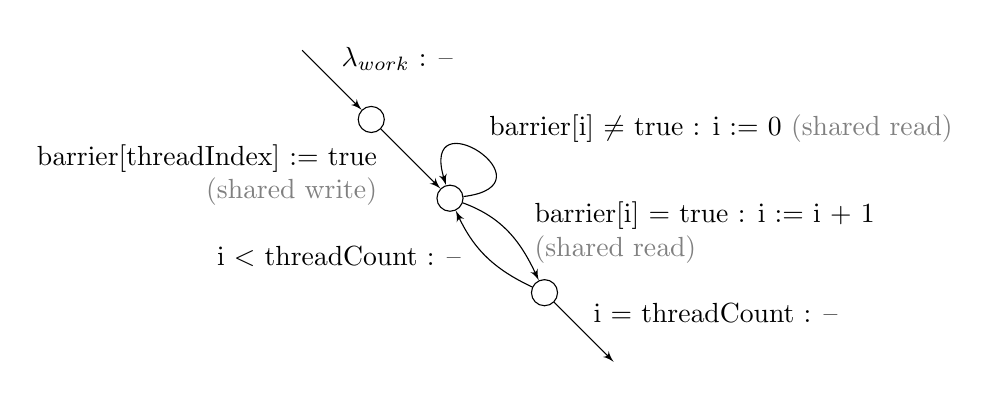
\begin{tikzpicture}[node distance = 2.0cm, auto]

% nodes
\node [o, draw=none] at ( 0   ,  0  ) (init) {};
\node [o]            at ( 1   , -1  ) (1)    {};
\node [o]            at ( 2   , -2  ) (2)    {};
\node [o]            at ( 3.2 , -3.2) (3)    {};
\node [o, draw=none] at ( 4.2 , -4.2) (done) {};

%  edges
\path [->] (init) edge                   node                          {$\lambda_{work}$ : --}                                       (1)
           (1)    edge   node [below left, pos=0.1, align=right] {barrier[threadIndex] := true \\ \color{gray}(shared write)}        (2)
           (2)    edge [loop, distance=1.2cm, out=7, in=107] node [above right] {barrier[i] $\ne$ true : i := 0 \color{gray}(shared read)} (2)
           (2)    edge [out=-20, in=115] node[right=0.2cm, align=left] {barrier[i] = true : i := i + 1 \\ \color{gray}(shared read)} (3)
           (3)    edge [out=155, in=-65] node[left=0.2cm]              {i $<$ threadCount : --}                                      (2)
           (3)    edge                   node                          {i = threadCount : --}                                        (done);

\end{tikzpicture}

	\caption{Control flow diagram of the B1 Barrier}
	\label{fig:model-b1}
\end{figure}

Initially each array element is set to false and the loop index to zero.
In comparison to the pseudocode the assignments are slightly different, but ultimately result in the same behaviour.

Deviating from the quantitative model, the functional model implements repetition and resetting by replacing the boolean array elements with counters. The principle is described in detail in Section~\ref{ssec:background-building-blocks}.
Additionally the functional model splits some of the transition into multiple transitions to allow for more interleaving and therefore reveal more potential errors in the protocol.

Splitting these transitions in the quantitative model would increase model size majorly, since the number of locations inflates the model's size exponentially in the number of threads. It is important not to merge multiple shared memory dependent transitions. Everything else influences timing only in a minor way.

%%%%%%%%%%
\paragraph{Dissemination Barrier}
\label{ssssec:analysis-modelchecking-modelling-dissemination}
The Dissemination Barrier (Figure~\ref{fig:pseudocode-dissemination}, Section~\ref{sssec:background-currently-used-distributed}), as a representative for distributed barrier algorithms, does not have shared memory. Therefore the CTMC model consists of one algorithm module per process and nothing else.

Figure~\ref{fig:model-dissemination} depicts the control flow diagram of the protocol.
The distance is initialised to one and each array element to false.
As in the two previous paragraphs a work period precedes the protocol.
The expressions \texttt{to} and \texttt{from} are shorthands for \texttt{processIndex $\pm$ dist (mod processCount)}.

\begin{figure}[htbp]
	\centering
	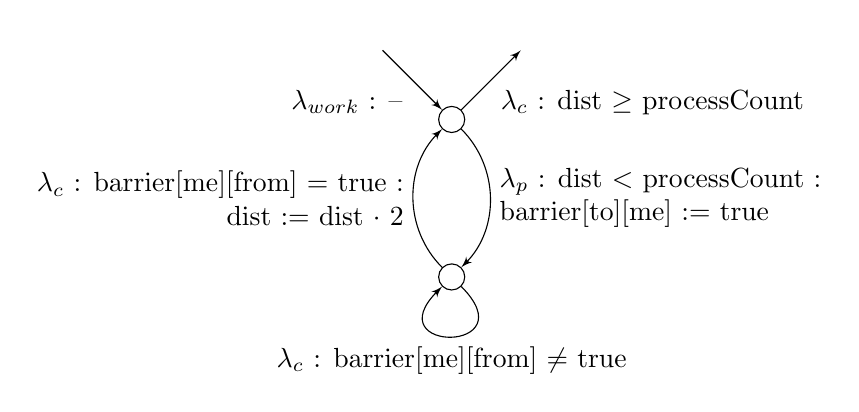
\begin{tikzpicture}[auto]

% nodes
\node [o, draw=none] at (  0 ,  0 ) (init) {};
\node [o]            at (  1 , -1 ) (1)    {};
\node [o]            at (  1 , -3 ) (2)    {};
\node [o, draw=none] at (  2 ,  0 ) (done) {};
%  edges
\path [->] (init) edge                  node [below left] {$\lambda_{work}$ : --} (1)

           (1)    edge node [below right] {$\lambda_c$ : dist $\ge$ processCount} (done)

           (1)    edge [out=-45, in=45] node [right, align=left] {$\lambda_p$ : dist $<$ processCount : \\ barrier[to][me] := true} (2)


           (2)    edge [loop, distance=1.2cm, out=315, in=225] node[below] {$\lambda_c$ : barrier[me][from] $\ne$ true} (2)

           (2)    edge [out=135, in=225] node[left, align=right]  {$\lambda_c$ : barrier[me][from] = true : \\ dist := dist $\cdot$ 2} (1);

\end{tikzpicture}

	\caption{Augmented Control flow diagram of the Dissemination Barrier}
	\label{fig:model-dissemination}
\end{figure}

Local operations take far less time than remote operations -- between ten to a thousand times usually. Therefore we assign the $\lambda_c$ (one processor clock cycle) to local operations.
The duration of a remote write (also called put) operation, which is strongly hard-ware dependent, is assumed to take 100 cycles. Therefore we assign $\lambda_p = \frac{1}{100}$ to each corresponding transition.

One could model the algorithm in more detail by splitting some of the transitions into multiple ones. We refrain from this to keep the model size at a manageable level.

In the CTMC model, resulting from unwinding this control flow diagram, a remote write operation is represented as a synchronised action. When a process executes a put, the target process then changes its local state accordingly.

The functional model includes repetition and resetting with counters instead of boolean variables as described in Section~\ref{ssec:background-building-blocks}.

%%%%%%%%%%
\paragraph{B2 Barrier}
\label{ssssec:analysis-modelchecking-modelling-b2}
The B2 Barrier, introduced in Section~\ref{ssec:new-b2}, is modelled as a composition of one algorithm module per process.

Figure~\ref{fig:model-b2} illustrates the control flow of the protocol.
Initially each bitset is empty and the loop index is set to \texttt{processIndex}.
The rates of operations are the same as for the Dissemination Barrier except that, instead of remote writing, we assign a rate of $\lambda_g = \frac{1}{100}$ to remote read (also called get) transitions.

\begin{figure}[htbp]
	\centering
	%
% does not 100% reflect the prism model
%

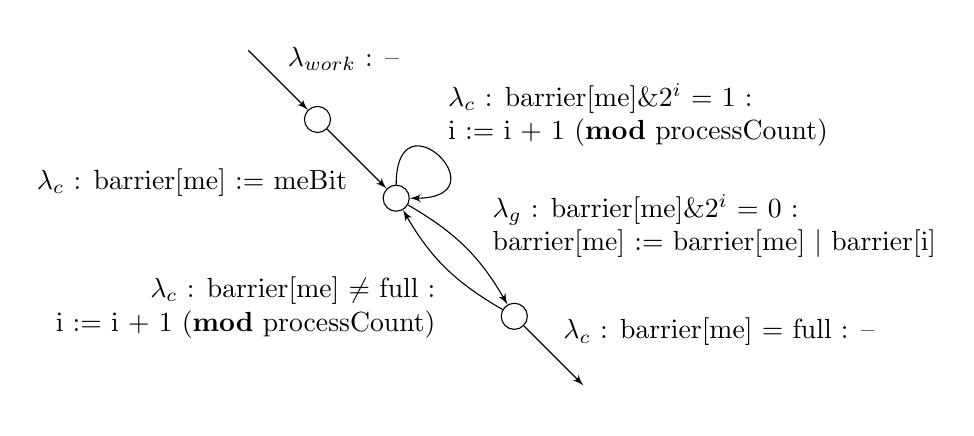
\begin{tikzpicture}[auto]

% nodes
\node [o, draw=none] at (   0 ,   0 )     (init) {};
\node [o]            at (   1.0 ,  -1.0 ) (1)    {};
\node [o]            at (   2.0 ,  -2.0 ) (2)    {};
\node [o]            at (   3.5 ,  -3.5 ) (3)    {};
\node [o, draw=none] at (   4.5 ,  -4.5 ) (done) {};

%  edges
\path [->]
  (init) edge                                      node [above right]             {$\lambda_{work}$ : --}                     (1)

  (1)    edge                                      node [below left]              {$\lambda_c$ : barrier[me] := meBit}        (2)

  (2)    edge [loop, distance=1.2cm, out=90, in=0] node [above right, align=left] {$\lambda_c$ : barrier[me]\&2$^i$ = 1 : \\ i := i + 1 (\textbf{mod} processCount)} (2)

  (2)    edge [out=-30, in=120] node [above right, pos=0.7, align=left] {$\lambda_g$ : barrier[me]\&2$^i$ = 0 : \\ barrier[me] := barrier[me] \textbar~barrier[i] } (3)

  (3)    edge [out=150, in=300]                    node [below left, align=right]  {$\lambda_c$ : barrier[me] $\ne$ full : \\ i := i + 1 (\textbf{mod} processCount)} (2)

  (3)    edge []                                   node [above right, align=left] {$\lambda_c$ : barrier[me] = full : --}     (done);


\end{tikzpicture}

	\caption{Augmented Control flow diagram of the B2 Barrier}
	\label{fig:model-b2}
\end{figure}

The functional model additionally includes repetition and resetting using the triple barrier approach explained in Section~\ref{ssec:background-building-blocks}.
Similar to previously presented models the functional model splits some of the transitions into multiple ones to allow for more interleaving. This way more potential errors can be revealed. The quantitative model refrains from splitting them to reduce the model's size.

%%%%%%%%%%%%%%%%%%%%
\subsubsection{Functional properties}
\label{sssec:analysis-modelchecking-functional-properties}
In this section we use the words \emph{thread} and \emph{process} interchangeably, because conditions of functional correctness apply to both shared and distributed memory protocols.

There are two basic conditions that every barrier protocol has to fulfill.
It has to properly synchronise threads and may not deadlock.
We express these two properties using the linear temporal logic (LTL).

\vspace{0.2cm}
\noindent \textbf{(A)} \emph{``A thread may only exit the barrier if all threads have entered it.''}
\begin{center}
	$\square ( \mathit{one\_left} \implies \mathit{all\_entered} )$
\end{center}

\vspace{0.2cm}
\noindent \textbf{(B)} \emph{``If all threads entered the barrier, each one leaves it in a finite amount of time.''}
\begin{center}
	$\square ( \mathit{all\_entered} \implies \lozenge \mathit{all\_left} )$
\end{center}

We use state predicates to describe sets of states with the intuitive meaning. For example $\mathit{one\_left}$ represents the set of states where at least one thread has passed the barrier.

We implemented each of the four chosen protocols in the modelling language Promela and verified properties A and B using the SPIN model checker.
Each barrier protocol fulfills both conditions.

%%%%%%%%%%%%%%%%%%%%
\subsubsection{Quantitative properties}
\label{sssec:analysis-modelchecking-quantitative-properties}
As in the previous section we use the words \emph{thread} and \emph{process} interchangeably, since some properties apply to both shared and distributed memory barrier protocols.

The section is divided into two parts. We first identify and formalise interesting quantitative properties of barrier protocols. Second we present the model checking results.

%%%%%%%%%%
\paragraph{Identification and formalisation}
\label{ssssec:analysis-modelchecking-quantitative-properties-identification}
There are a number of interesting questions to ask about barrier protocols. First let us enumerate what we can quantify.

Measuring time is obviously of great interest to us. We want to count how many processor clock cycles certain operations take. In order to measure cycles, we assign a state reward of 1 to each state. The accumulated reward is then the desired value.

Another interesting quantity to measure is energy consumption (unit joule) and its rate, measured in Watt (joule per second).
To measure these, we use a mix of transition and state rewards.
The following, very limited assumptions are based on a sample measurement presented in Section~\ref{ssec:energy-measurement}.
We assume a processor clock rate of 2.5 GHz to convert between seconds and cycles.
We assume the processor to consume 11 Watts as a baseline.
Local operations are assigned no reward.
For shared memory protocols we assign a cost of 2 nanojoules (nJ) to each instantaneous memory operation and 200 nanojoules to each slow memory operation.
For distributed memory we assume a cost 200 nanojoules per remote memory operation and 2 nanojoules for each local memory operation.

For distributed memory protocols we are also interested in the number of remote operations issued. To obtain this measure we assign a transition reward of 1 to each corresponding transition.

Having listed the three measures we want to quantify, we now consider the points in time when we want to measure.
There are four of these: the moment when the first (A), and the last (B), thread enters the barrier, and the instant when the first (C), and last (D), thread leaves the barrier.
For the shared memory barriers we additionally consider the moment when the writing phase ends (W), i.e. when the last thread finished writing.
Since the Dissemination Barrier consists of multiple rounds, we are also interested in measuring at the end of each round (R$i$). That is the point in time when the last thread leaves round $i$.

Formalising the preceding enumeration we present the list of properties used for model checking.

\vspace{0.2cm}
\noindent \textbf{(A)} \emph{``Average reward until any one thread entered the barrier''}
\begin{center}
	$\mathrm{ReaRew}( \mathit{one\_entered} )$
\end{center}

\vspace{0.2cm}
\noindent \textbf{(B)} \emph{``Average reward until all threads entered the barrier''}
\begin{center}
	$\mathrm{ReaRew}( \mathit{all\_entered} )$
\end{center}

\vspace{0.2cm}
\noindent \textbf{(C)} \emph{``Average reward until any one thread left the barrier''}
\begin{center}
	$\mathrm{ReaRew}( \mathit{one\_left} )$
\end{center}

\vspace{0.2cm}
\noindent \textbf{(D)} \emph{``Average reward until every thread left the barrier''}
\begin{center}
	$\mathrm{ReaRew}( \mathit{all\_left} )$
\end{center}

\vspace{0.2cm}
\noindent \textbf{(W)} \emph{``Average reward until every thread finished writing''}
\begin{center}
	$\mathrm{ReaRew}( \mathit{all\_done\_writing} )$
\end{center}

\vspace{0.2cm}
\noindent \textbf{(R$i$)} \emph{``Average reward until every thread left round $i$''}
\begin{center}
	$\mathrm{ReaRew}( \mathit{all\_left\_round_{i}} )$
\end{center}

\noindent The state predicates have the intuitive meaning. For example $\mathit{all\_left\_round_{i}}$ describes the set of states where all threads passed round $i$.
We additionally consider combinations of the above properties, for example D minus B, which measures the average reward accumulated between the last thread entering the barrier and the last thread leaving the barrier.

There are two main parameters to variate for the measurements. The first one is the number of threads participating in the barrier synchronisation. Because the model size grows exponentially in the number of threads we are mostly restricted to thread counts of up to four.
The second value to variate is the initial work period's rate. By changing the work rate we can consider scenarios where threads arrive in smaller and larger intervals.

%%%%%%%%%%
\paragraph{Evaluation}
\label{ssssec:analysis-modelchecking-quantitative-properties-evaluation}
\begin{itemize}
	\item 
\end{itemize}

%%%%%
\subparagraph{Shared memory barriers}
\label{sssssec:analysis-modelchecking-quantitative-properties-evaluation-shared}
\begin{itemize}
	\item work = 100. Expected time it takes a thread to arrive at the barrier is 100 cycles.
	\item last to last, last to first Figure~\ref{fig:c1-time-work-100-B-C-D}
		\begin{figure}[htbp]
			\centering
			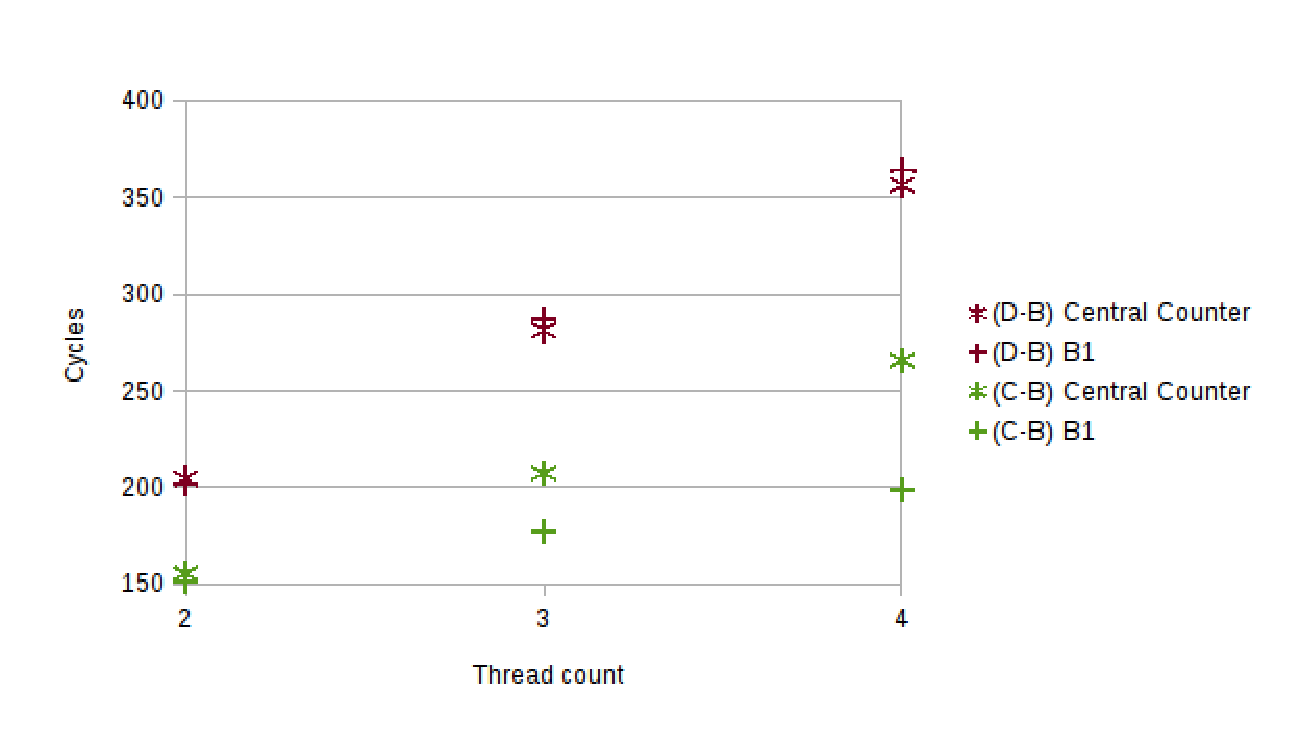
\includegraphics[width=10cm]{charts/c1-time-work-100-B-C-D}
			\caption{Expected execution time}
			\label{fig:c1-time-work-100-B-C-D}
		\end{figure}
		\begin{itemize}
			\item both barriers similarly fast when considering the last one to finish
			\item B1 is faster for the first one to leave
		\end{itemize}
	\item distribution of total time and energy spent: Figure~\ref{fig:c1-work-100-partition}
		\begin{figure}[htbp]
			\centering
			\begin{minipage}{0.53\linewidth}
				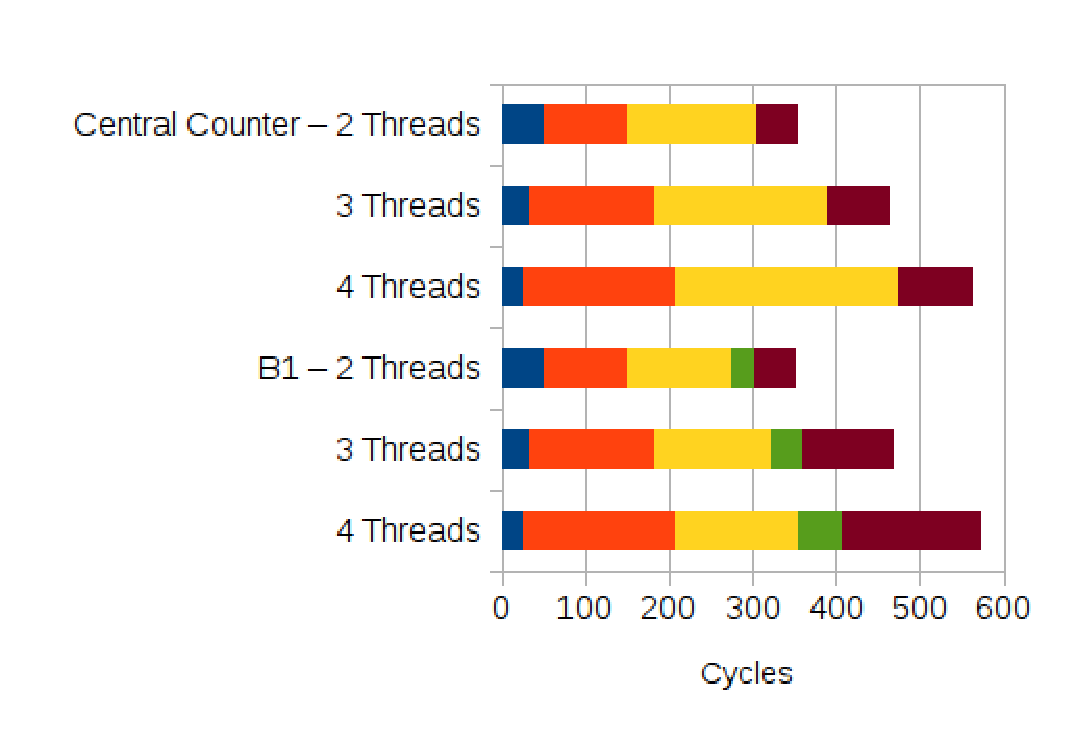
\includegraphics[height=4.3cm]{charts/c1-time-work-100-partition}
			\end{minipage}
			\begin{minipage}{0.46\linewidth}
				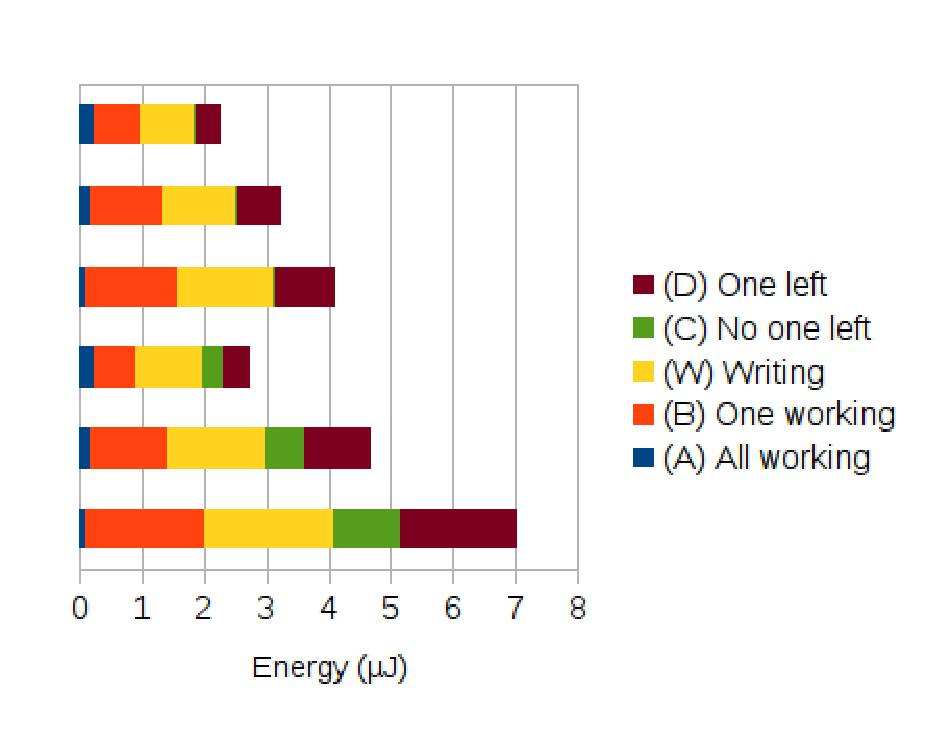
\includegraphics[height=4.3cm]{charts/c1-energy-work-100-partition}
			\end{minipage}
			\caption{Distribution of total time spent and energy consumed}
			\label{fig:c1-work-100-partition}
		\end{figure}
	\item time
		\begin{itemize}
			\item stacked fashion. Including the time of the previous bar.
			\item the initial work distribution is the same for all processes and protocols
			\item cc: first thread leaves a few cycles after writing is done. Because the last one to write its value will likely immediately read the completed barrier and leave.
			\item from the moment the first thread leaves, all threads only read. No one writes anymore.
			\item writing, as expected, takes longer for Central Counter and reading takes longer for the B1 Barrier
			\item all parts take longer with increasing thread count, since CTMC semantic (described in Section~\ref{sssec:analysis-modelchecking-preliminaries}) makes a transition get an exit rate of the sum of the rates of all enabled transitions.
			\item in particular, assume you have $n$ interleaved modules (or concurrent threads of execution) where one transition in each module is enabled. The exit rate of the first transition to be triggered is then  $n \cdot \lambda$. The expected time of a parallel execution of all transitions is $\sum_{i=1}^{n} \frac{1}{i \cdot \lambda}$ time rather than $\frac{1}{\lambda}$.
			\item for example the expected number of cycles for the first process to enter is $\approx \frac{100}{n}$. The last one is finished working after $\approx$ 150, 183 and 208 cycles, for two, three and four processes.
			\item Especially reading for Central Counter (2: 50, 3:75, 4:92 cycles). Normally this period is expected to be nearly the same for all thread counts.
			\item writing for the B1 Barrier is expected to take less time than shown here (100 across the board instead of 2:125, 3:138, 4:146), for the same reason as reading takes longer as expected for the Central Counter Barrier.
		\end{itemize}
	\item energy
		\begin{itemize}
			\item similar to time
			\item the B1 Barrier needs more energy. Because it performs more shared memory operations and more local operations in the same amount of time, where the Central Counter Barrier spends considerable time waiting for atomic operations to finish.
			\item Central Counter's energy scales similarly to time.
			\item amount of energy for the B1 Barrier grows faster than time needed.
			\item the B1 Barrier spends considerable energy from the last commitment to first leaving the barrier.
		\end{itemize}
	\item rate of power consumption per protocol phase: Figure~\ref{fig:c1-power-work-100}
		\begin{figure}[htbp]
			\centering
			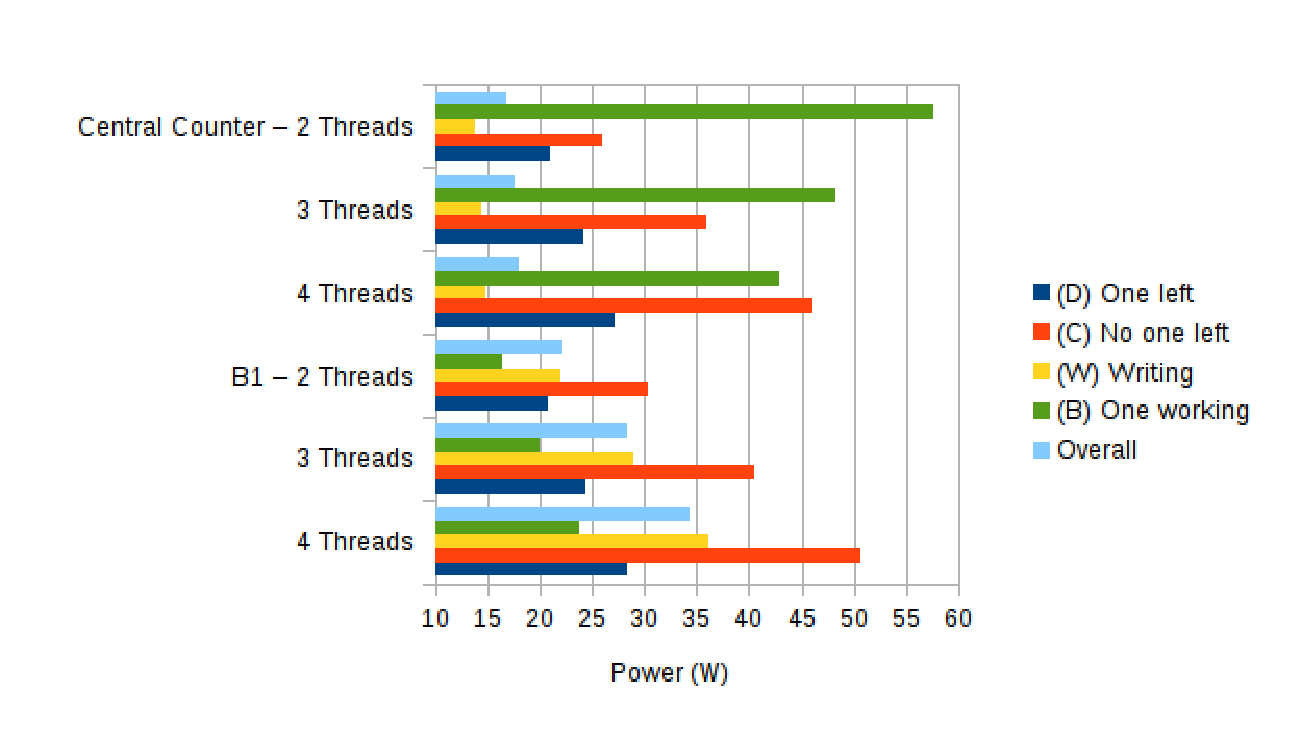
\includegraphics[width=10cm]{charts/c1-power-work-100}
			\caption{Rate of energy consumption for each phase}
			\label{fig:c1-power-work-100}
		\end{figure}
		\begin{itemize}
			\item same partitioning as the previous figure.
			\item (A) all working has 11W - the baseline.
			\item overall low for Central Counter (16-18.3W), B1 (19.4 - 30.6)
			\item writing considerably higher for rs, because quicker and more shared memory operations.
			\item no one left: cc: high because very very short, rs: high because many shared reads across many threads.
			\item one left similar because cc: shared reads, rs: shared reads, and local reads.
		\end{itemize}
	\item reading vs writing: Figure~\ref{fig:c1-time-work-100-percent}
		\begin{figure}[htbp]
			\centering
			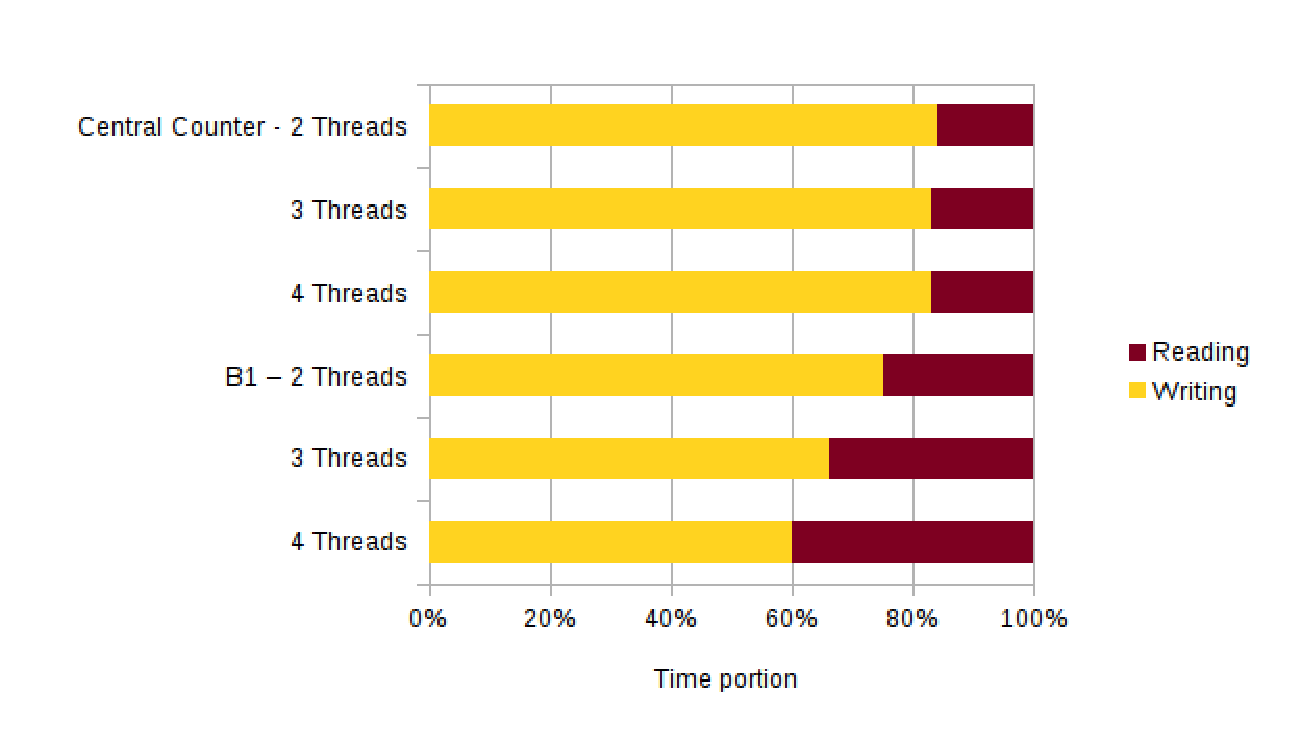
\includegraphics[width=10cm]{charts/c1-time-work-100-percent}
			\caption{Time spent reading versus writing}
			\label{fig:c1-time-work-100-percent}
		\end{figure}
		\begin{itemize}
			\item writing is from (A) to (W). Reading is from (W) to (D).
			\item with increasing thread count there is a shift from writing to reading in execution time.
		\end{itemize}
	\item work=1000. Still very small. (According to \cite{rab00} at a barrier each process spends on average 8194 CPU cycles idly\footnote{1813 microseconds accumulated idle time at 450MHz on 99.6 processes})
	\item last to last, last to first Figure~\ref{fig:c1-time-work-1000-B-C-D}
		\begin{figure}[htbp]
			\centering
			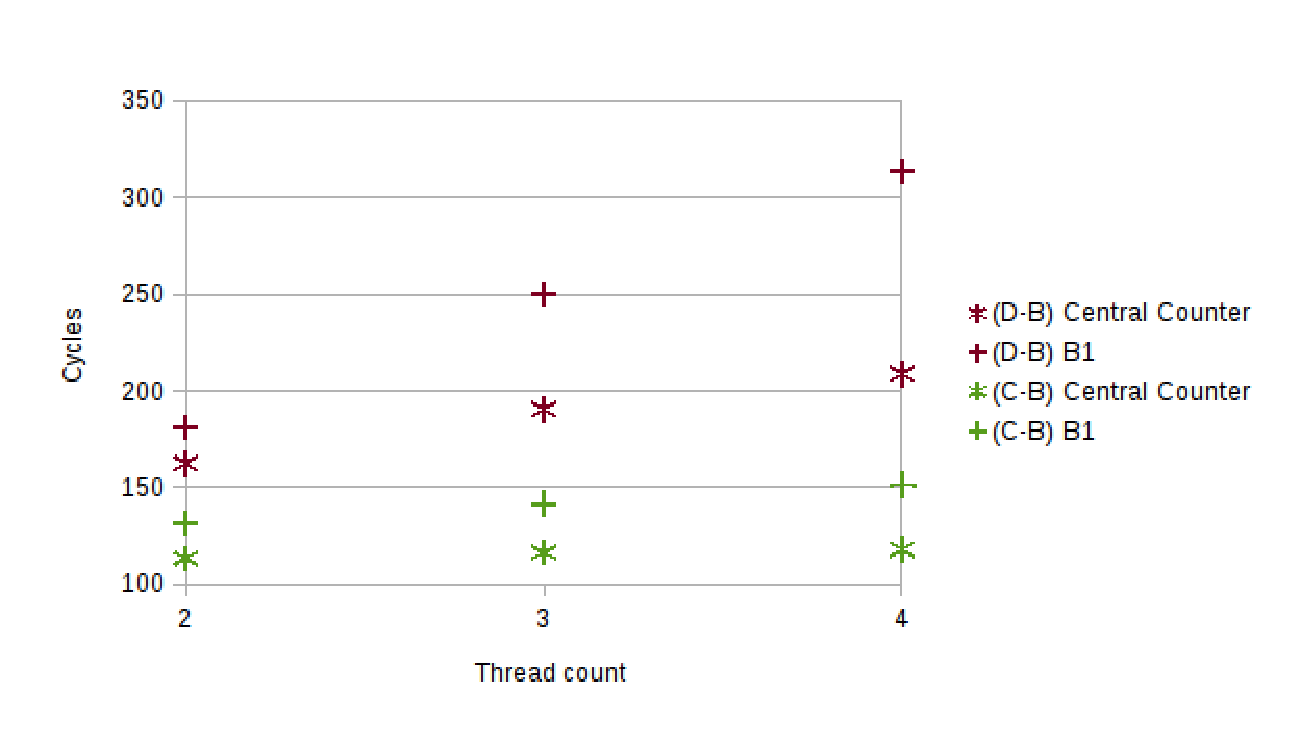
\includegraphics[width=10cm]{charts/c1-time-work-1000-B-C-D}
			\caption{Expected execution time}
			\label{fig:c1-time-work-1000-B-C-D}
		\end{figure}
		\begin{itemize}
			\item very different picture.
			\item Central Counter faster in all respects.
			\item probability of a thread trying to write while no one is writing at the moment increases due to the larger working period distribution. Writes for the B1 Barrier tend to be serialized for the same reason, but B1 still reads longer.
			\item time for one thread from entry to exit converges to one atomic op + a few cycles. 105 cycles for Central Counter.
		\end{itemize}
	\item distribution of total time and energy spent: Figure~\ref{fig:c1-work-1000-partition}
		\begin{figure}[htbp]
			\centering
			\begin{minipage}{0.53\linewidth}
				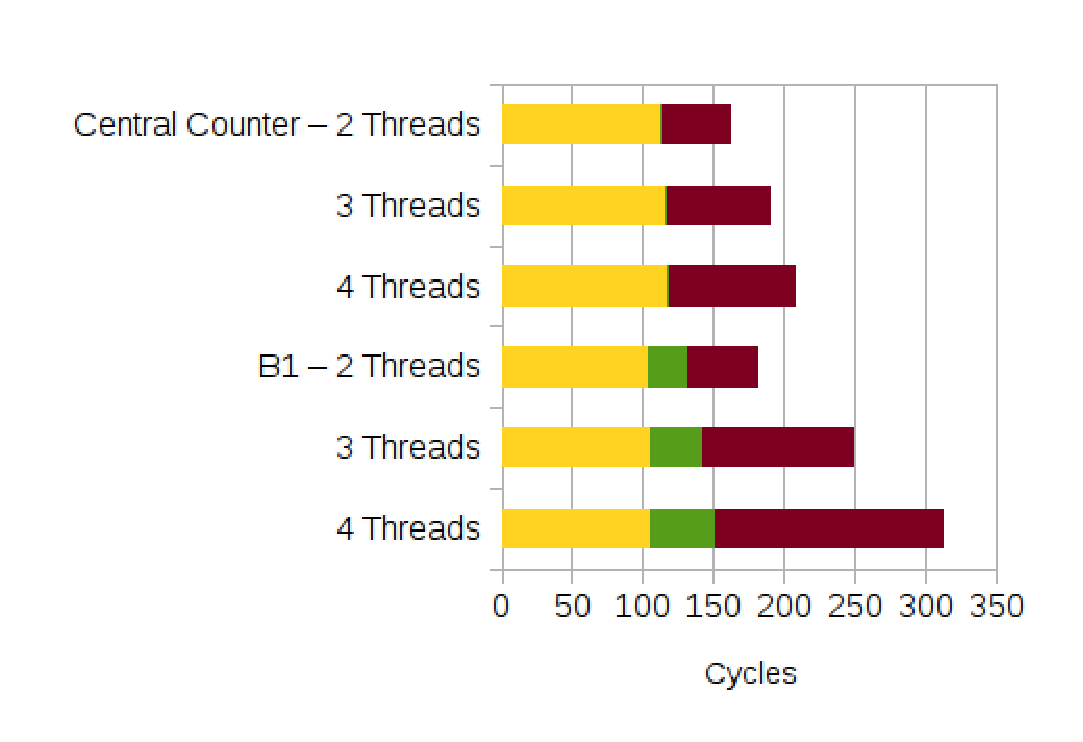
\includegraphics[height=4.3cm]{charts/c1-time-work-1000-partition}
			\end{minipage}
			\begin{minipage}{0.46\linewidth}
				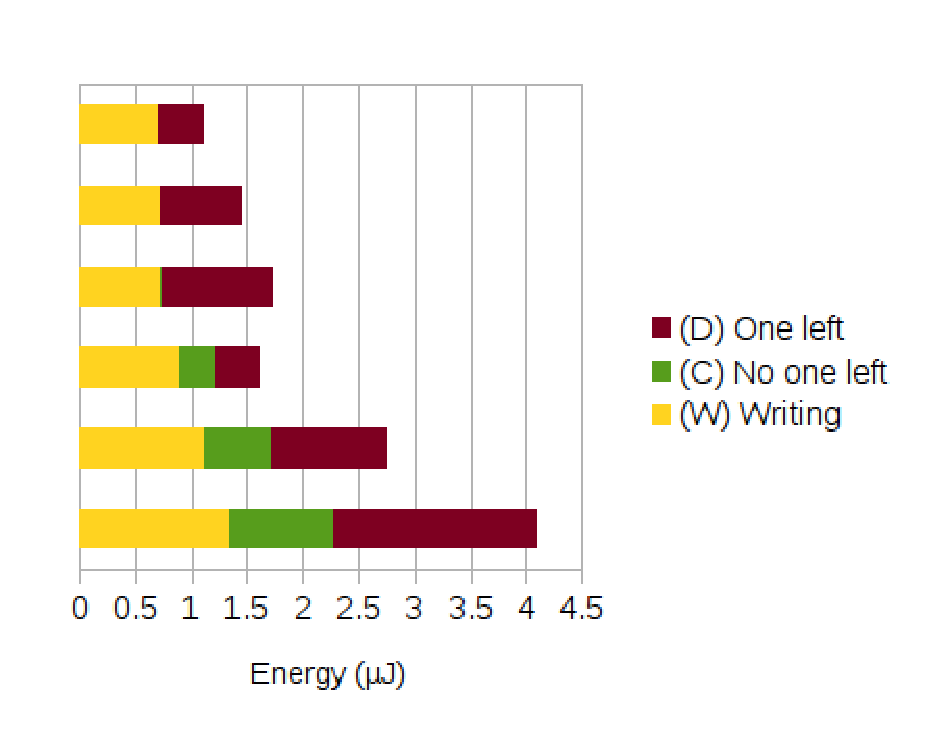
\includegraphics[height=4.3cm]{charts/c1-energy-work-1000-partition}
			\end{minipage}
			\caption{Distribution of total time spent and energy consumed}
			\label{fig:c1-work-1000-partition}
		\end{figure}
		\begin{itemize}
			\item Excluding (A) and (B) since they are large in comparison to the barrier
		\end{itemize}
	\item time
		\begin{itemize}
			\item as expected
		\end{itemize}
	\item energy
		\begin{itemize}
			\item writing is constant across multiple threads because the atomic op forbids reading the variable thus there is few busy waiting, whereas B1 is constantly polling. And the amount increases with increasing thread count.
		\end{itemize}
	\item rate of power consumption per protocol phase: Figure~\ref{fig:c1-power-work-1000}
		\begin{figure}[htbp]
			\centering
			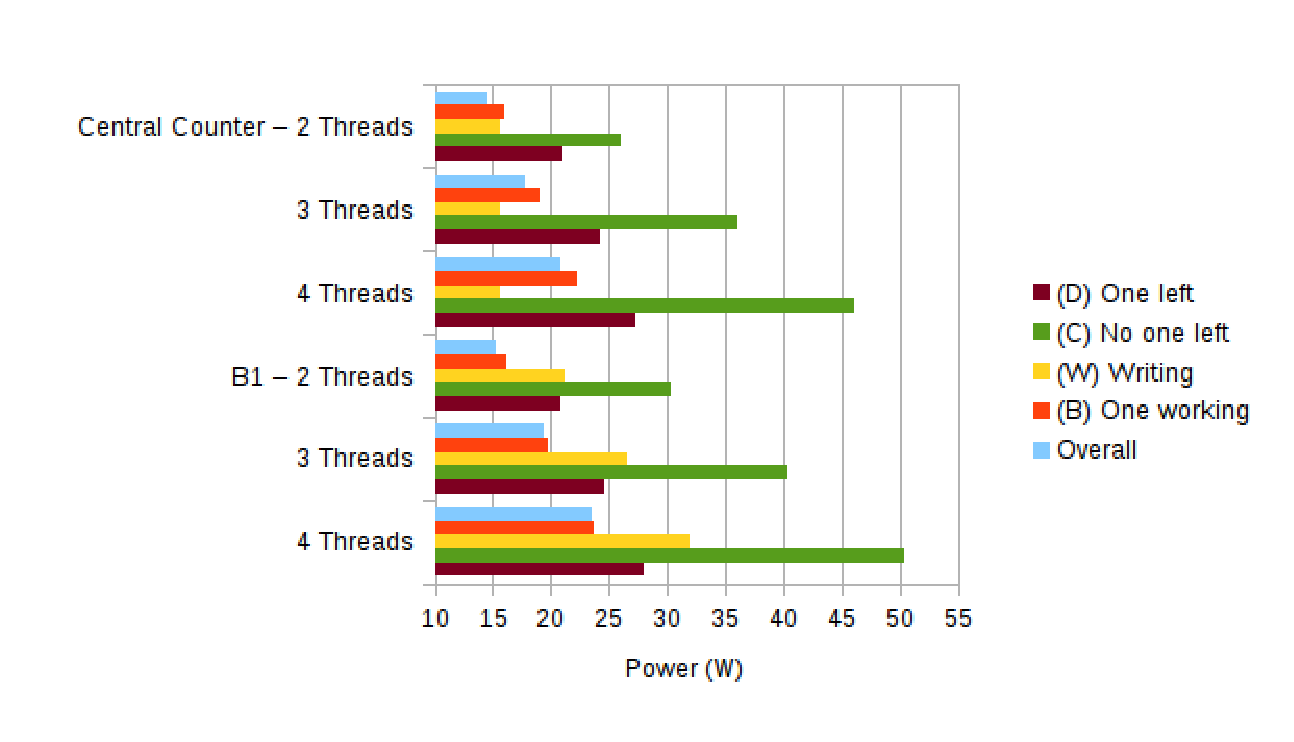
\includegraphics[width=10cm]{charts/c1-power-work-1000}
			\caption{Rate of energy consumption for each phase}
			\label{fig:c1-power-work-1000}
		\end{figure}
		\begin{itemize}
			\item more even. (1) longer work period. (2) cc and rs use similarly many shared and local operations (due to busy waiting) in the reading phase ((D) one left). Energy usage is dominated by busy waiting of threads.
			\item the B1 Barrier can catch up considerably. (cc:14.6-20.9, rs:15.3-23.5)
		\end{itemize}
	\item with larger and more realistic, since 1000 cycles is still very few, work periods this yields a series of writing operations for both algorithms, and a little more time spent reading for the B1 Barrier.
\end{itemize}

%%%%%
\subparagraph{Distributed memory barriers}
\label{sssssec:analysis-modelchecking-quantitative-properties-evaluation-distributed}
\begin{itemize}
	\item work = 100
	\item distribution of total time spent and total energy consumed: Figure~\ref{fig:d2-work-100-partition}
		\begin{figure}[htbp]
			\centering
			\begin{minipage}{0.54\linewidth}
				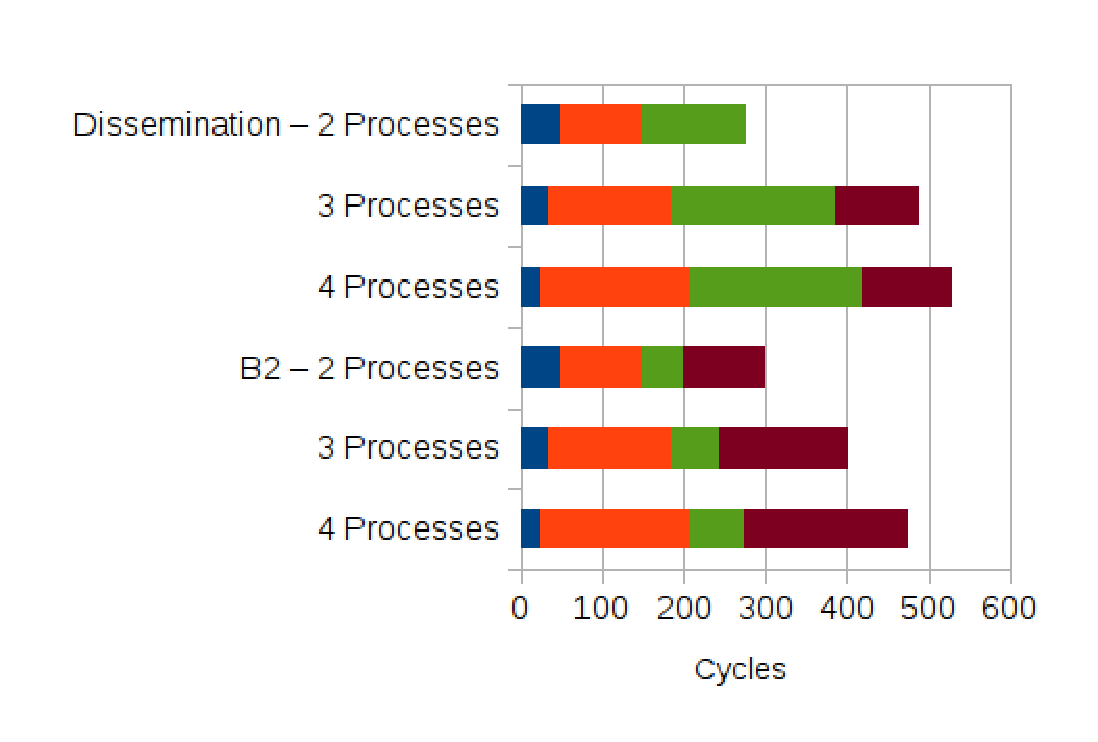
\includegraphics[height=4.3cm]{charts/d2-time-work-100-partition}
			\end{minipage}
			\begin{minipage}{0.45\linewidth}
				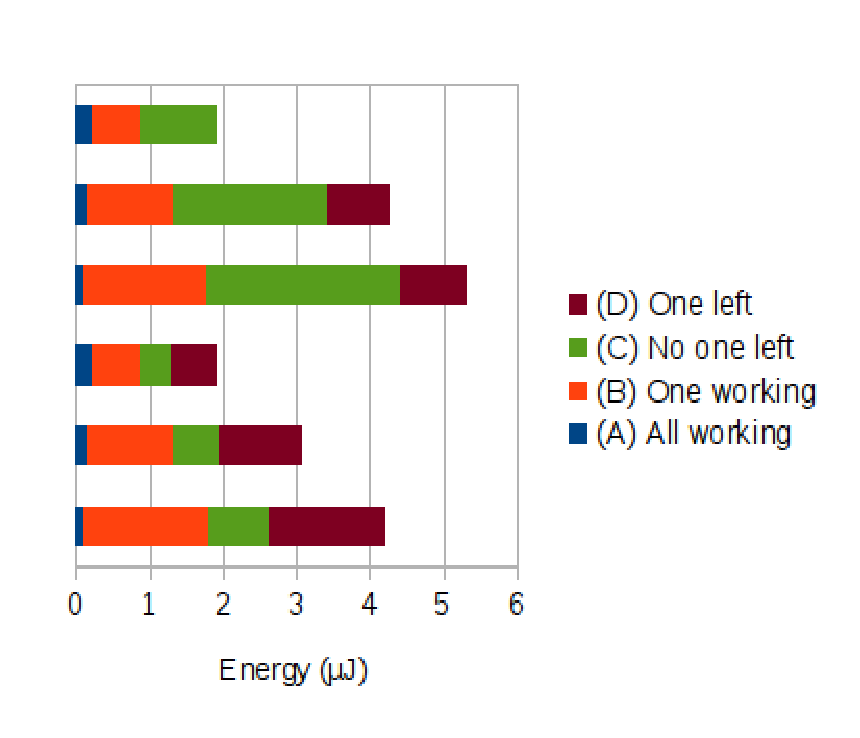
\includegraphics[height=4.3cm]{charts/d2-energy-work-100-partition}
			\end{minipage}
			\caption{Distribution of total time spent and energy consumed}
			\label{fig:d2-work-100-partition}
		\end{figure}
		\begin{itemize}
			\item the B2 Barrier is quicker for process counts over two
			\item Dissemination finishes 23 cycles earlier than the B2 Barrier for 2 processes because remote write can be executed during the work period of the other process, whereas the B1 Barrier still needs to execute 2 remote reads after the last process entered the barrier.
			\item rf: first one to leave unrealistic. Should not be quicker than 100 cycles. CTMC exit rate calculation.
			\item more time between first and last to leave.
			\item last and first exit at almost the same time for Dissemination, because when the second arrives and writes his part into the remote peers memory both will quickly exit. This cannot happen for processes since when the first leaves there might still be pending remote writes.
			\item energy consumption similar to time spent in proportion
		\end{itemize}
	\item Dissemination: distribution of total time spent and energy consumed: Figure~\ref{fig:d-work-100-partition}
		\begin{figure}[htbp]
			\centering
			\begin{minipage}{0.43\linewidth}
				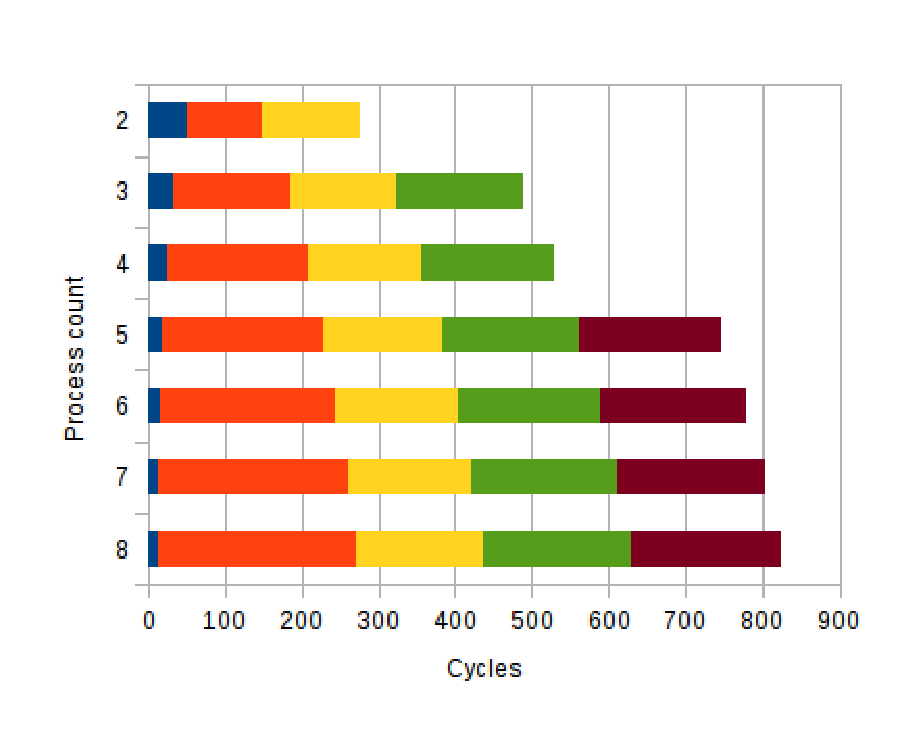
\includegraphics[height=4.2cm]{charts/d-time-work-100-partition}
			\end{minipage}
			\begin{minipage}{0.56\linewidth}
				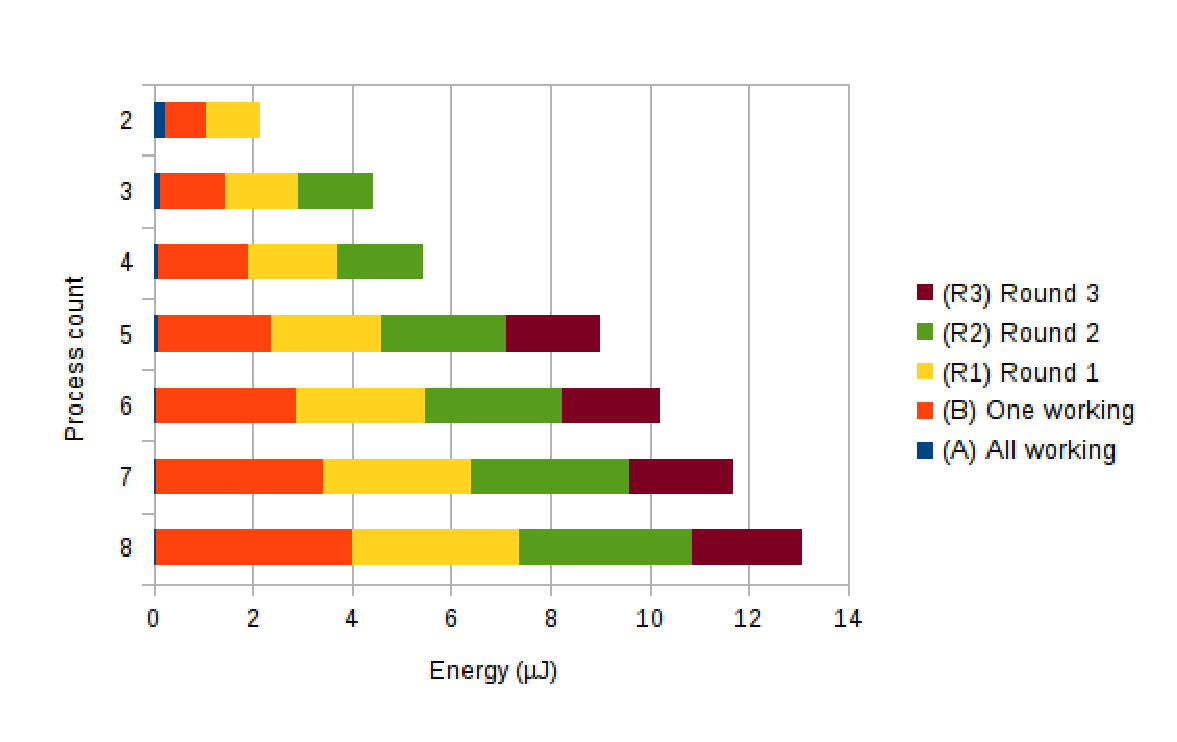
\includegraphics[height=4.2cm]{charts/d-energy-work-100-partition}
			\end{minipage}
			\caption{Distribution of total time spent and energy consumed for the Dissemination Barrier}
			\label{fig:d-work-100-partition}
		\end{figure}
		\begin{itemize}
			\item stair-esque running time due to $\lceil \log_2 \mathit{processCount} \rceil$ number of rounds. During those rounds remote writes are issued concurrently.
			\item unfavourable for non-power-of-two processes counts. Ref to Section~\ref{sssec:analysis-general-distributed}
			\item slight increase in per-round execution time with number of processes is result of CTMC interleaving semantics. This behaviour is realistic, because resource contention for remote writes and + non-uniform distribution durations for those writes, but we didn't specifically model this.
			\item energy consumption increase per round a bit larger than runtime increase. This is partly because more remote operations are issued as described in Section~\ref{ssssec:analysis-modelchecking-modelling-dissemination}. And partly because one more process is locally spinning before entering a new round.
		\end{itemize}
	\item rate of power consumption per phase: Figure~\ref{fig:d2-power-work-100}
		\begin{figure}[htbp]
			\centering
			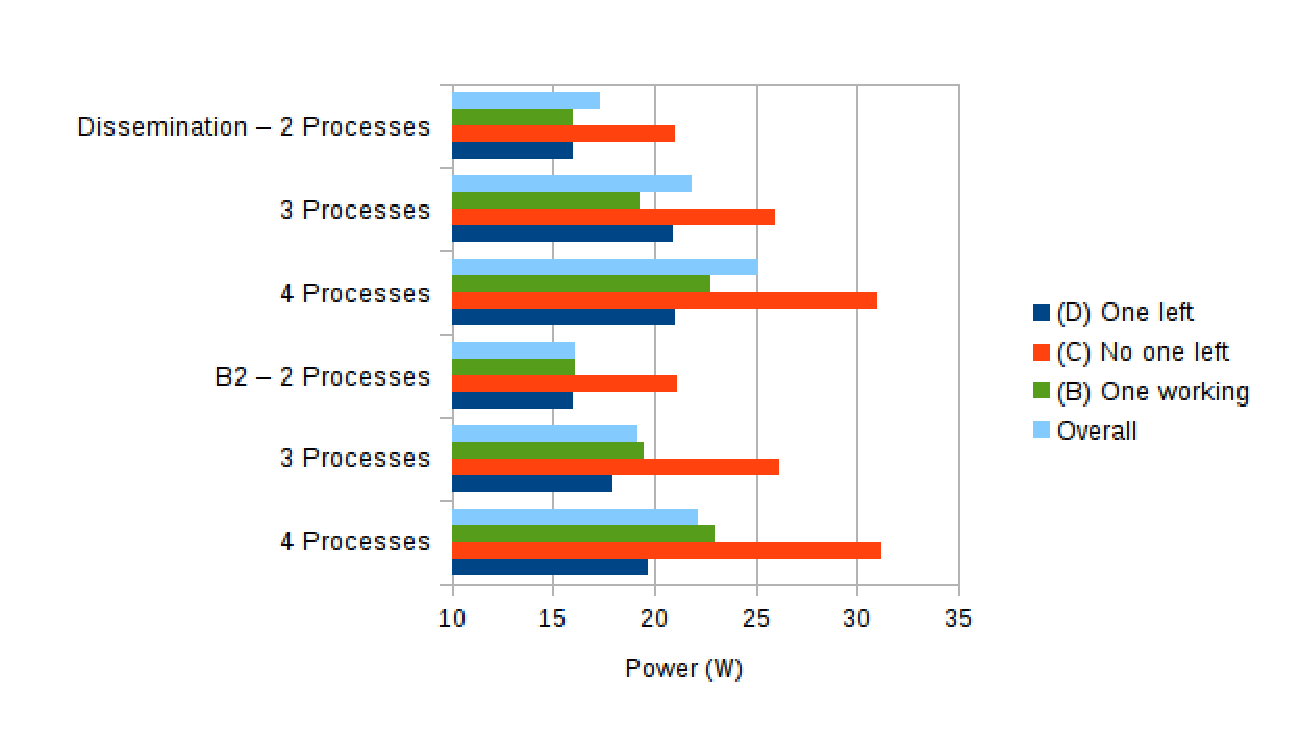
\includegraphics[width=10cm]{charts/d2-power-work-100}
			\caption{Rate of energy consumption for each phase}
			\label{fig:d2-power-work-100}
		\end{figure}
		\begin{itemize}
			\item All phases except the last are very similar.
			\item largely because comparing number of local and remote operations issued to the rewards given for these operations the amount of energy consumed is expected to be similar.
			\item Dissemination issues less remote operations, but due to local wait spinning a lot of local operations, the B2 Barrier on the other hand polls remotely.
			\item in the last phase the B2 Barrier draws less power because it takes a lot more time for a little more energy to be consumed.
			\item overall the B2 Barrier performs slightly better.
		\end{itemize}
	\item longer work period. work=1000
	\item distribution of total time spent and energy consumed: Figure~\ref{fig:d2-work-1000-partition}
		\begin{figure}[htbp]
			\centering
			\begin{minipage}{0.54\linewidth}
				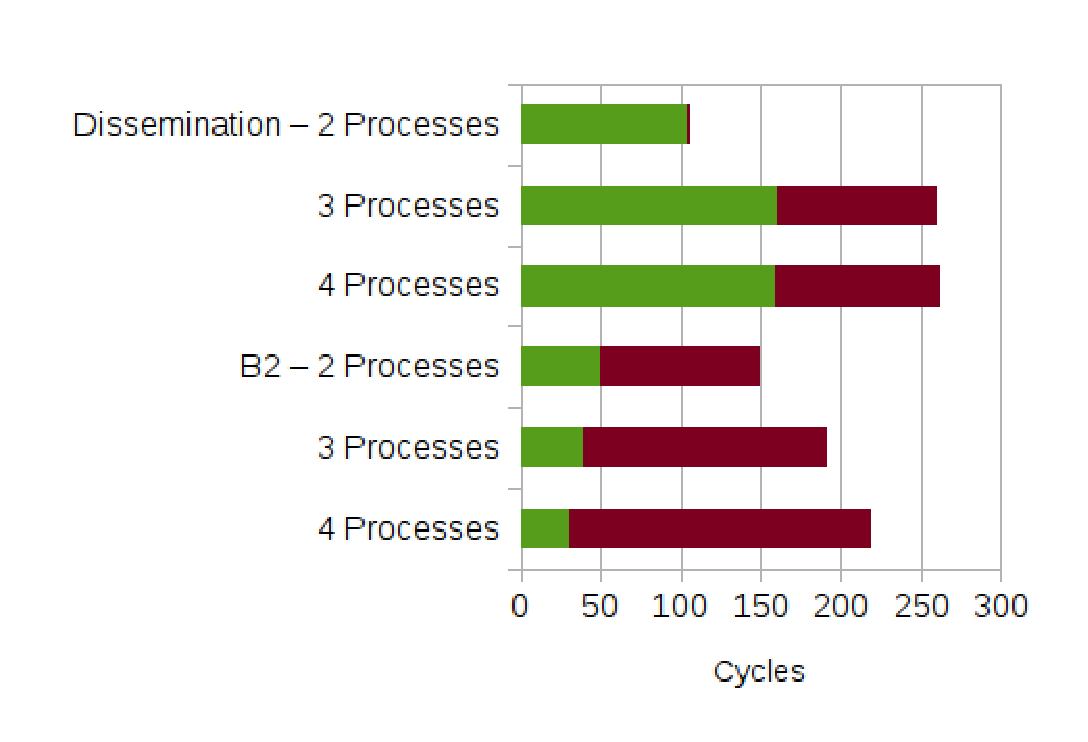
\includegraphics[height=4.3cm]{charts/d2-time-work-1000-partition}
			\end{minipage}
			\begin{minipage}{0.45\linewidth}
				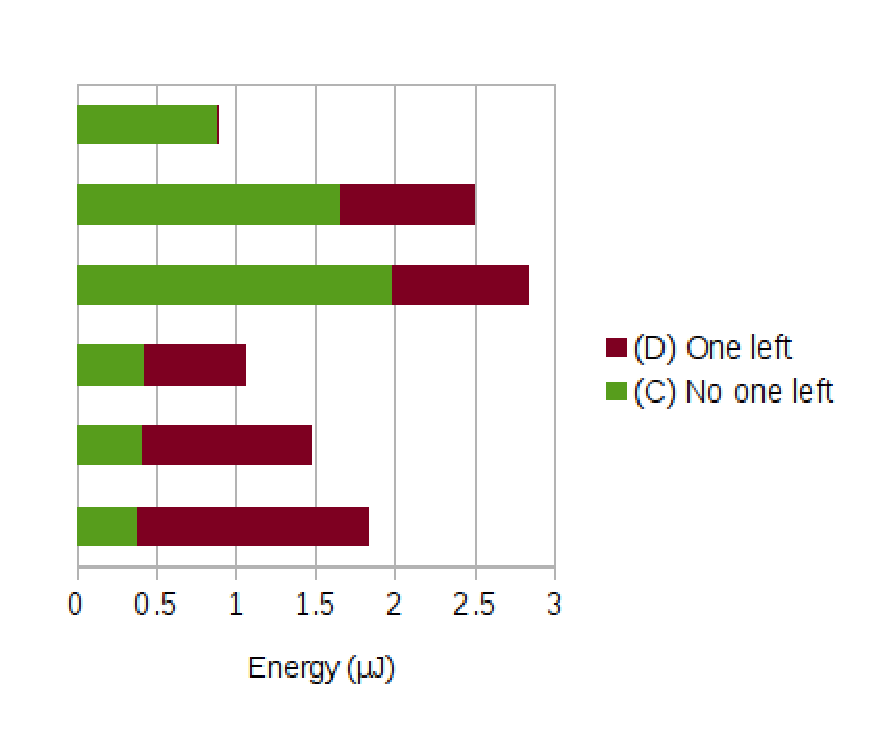
\includegraphics[height=4.3cm]{charts/d2-energy-work-1000-partition}
			\end{minipage}
			\caption{Distribution of total time spent and energy consumed}
			\label{fig:d2-work-1000-partition}
		\end{figure}
		\begin{itemize}
			\item excluding (A) and (B) because long.
			\item first one to leave for rf unrealistic as in Figure~\ref{fig:d2-work-100-partition}
		\end{itemize}
	\item Dissemination: distribution of total time spent and energy consumed: Figure~\ref{fig:d-work-1000-partition}
		\begin{figure}[htbp]
			\centering
			\begin{minipage}{0.43\linewidth}
				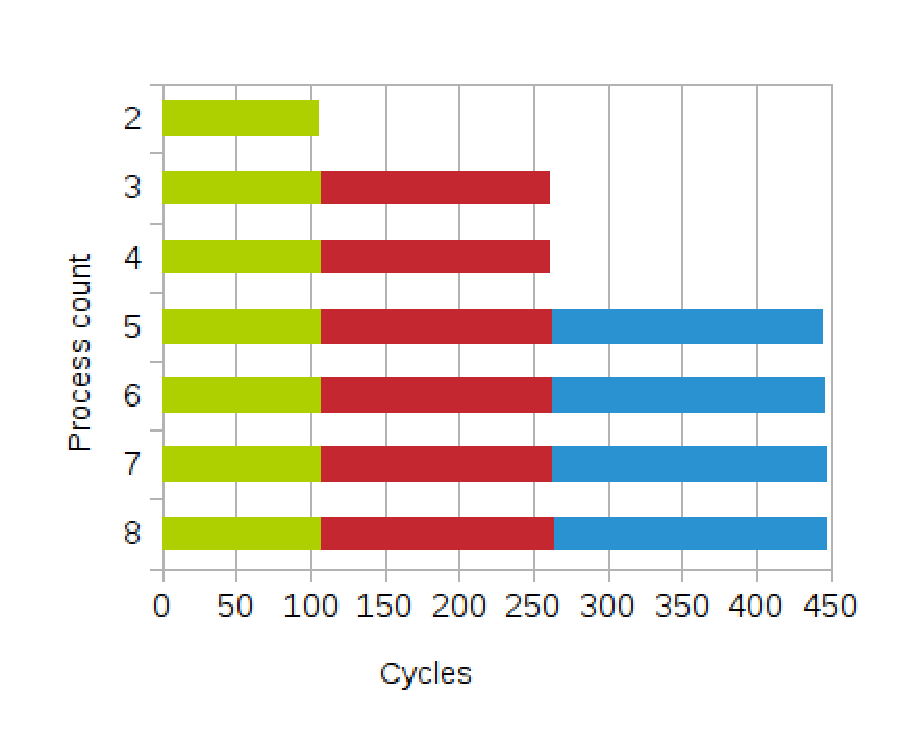
\includegraphics[height=4.2cm]{charts/d-time-work-1000-partition}
			\end{minipage}
			\begin{minipage}{0.56\linewidth}
				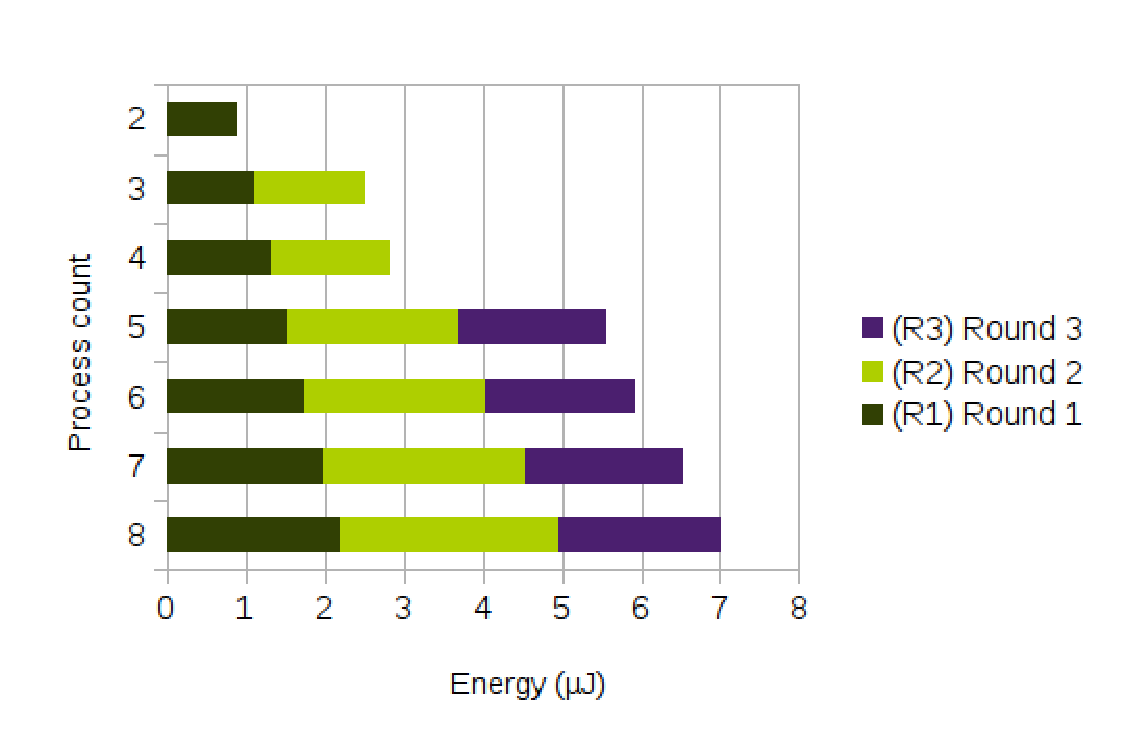
\includegraphics[height=4.2cm]{charts/d-energy-work-1000-partition}
			\end{minipage}
			\caption{Distribution of total time spent and energy consumed for the Dissemination Barrier}
			\label{fig:d-work-1000-partition}
		\end{figure}
		\begin{itemize}
			\item as expected
			\item In comparison to Figure~\ref{fig:d-work-100-partition} there is almost no additional time cost per process associated. CTMC semantic effect diminishes because the remote writes in the rounds are approximately serial. Therefore a write is oftentimes activatable at the same time as other processes are repeatedly executing local reads. The expected time such a write takes is then $\approx 100$ CPU cycles.
			\item the durations for the rounds are related to the progress explanation in Section~\ref{sssec:analysis-general-distributed}. When the last process arrives at the barrier, exactly one remote write is needed to finish round one, two more writes are needed to finish round two and four writes are needed to finish the third round. Therefore, and because of CTMC interleaving semantics, approximately 100, 150 and 183 cycles are needed to finish rounds one, two and three.
			\item Energy usage increases with each additional progress for the same reasons as in Figure~\ref{fig:d-work-100-partition}
			\item progress problem.
			\item there is a fixed cost for each additional round in the Dissemination Barrier.
			\item due to model checking limitations (a very large state space), we cannot quantify beyond four processes, i.e. two rounds.
			\item as shown in Figure~\ref{fig:d-work-1000-partition} the B2 Barrier is indeed quicker.
			\item in relation to the results from work period 100, the B2 Barrier could not increase its headway at work period 1000.
			\item this does not necessarily mean that the progress problem does not exist. It might for example mean that the B2 Barrier does not handle this situation as efficiently as we expected or that it did better than we expected for the 100 cycle work period case. Either way it is definitely possible to be generally faster than the Dissemination Barrier is for this scenario.
		\end{itemize}
	\item rate of power consumption per phase: Figure~\ref{fig:d2-power-work-1000}
		\begin{figure}[htbp]
			\centering
			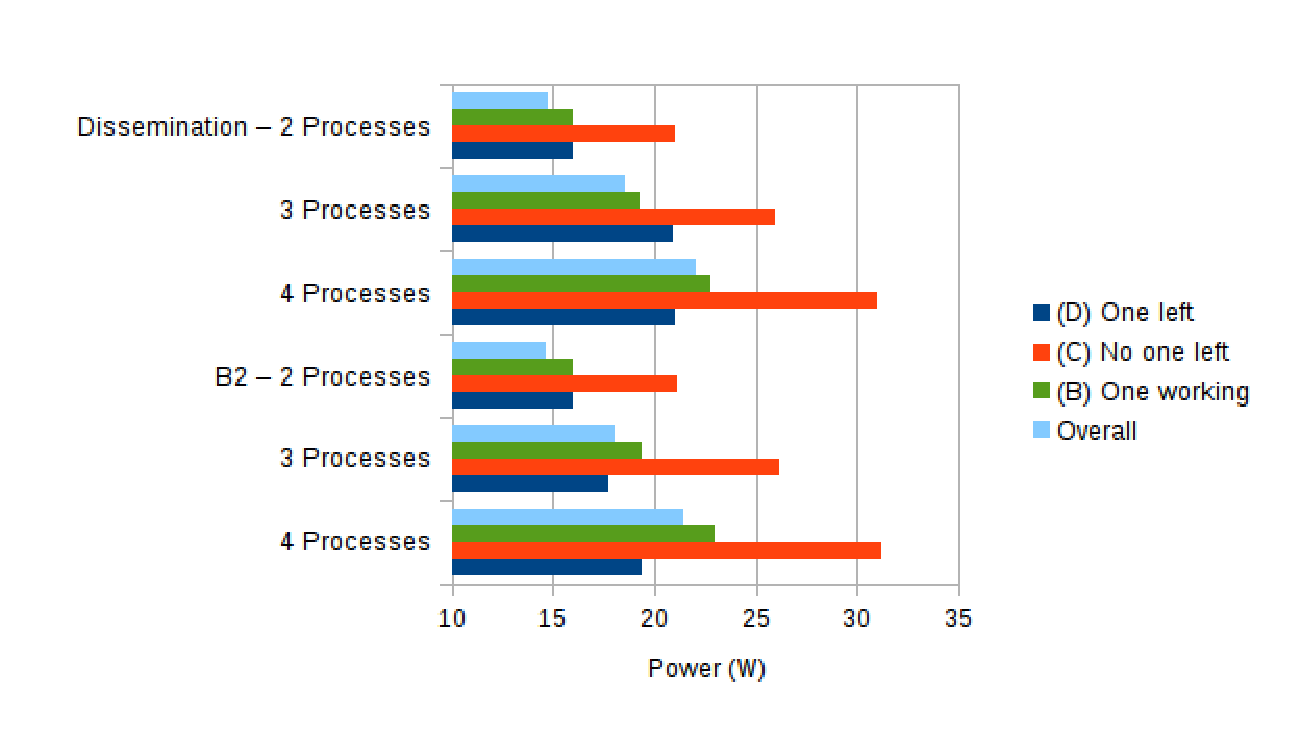
\includegraphics[width=10cm]{charts/d2-power-work-1000}
			\caption{Rate of energy consumption for each phase}
			\label{fig:d2-power-work-1000}
		\end{figure}
		\begin{itemize}
			\item overall power consumption slightly lower because of the 1000 cycle work period.
			\item everything else similar to Figure~\ref{fig:d2-power-work-100}.
		\end{itemize}
	\item number of remote transfers
		\begin{itemize}
			\item remote transfer is a generic term including remote reads and remote writes.
			\item fixed for Dissemination as explained in Section~\ref{sssec:analysis-general-distributed}. $n \cdot \lceil \log _2~n \rceil$
			\item number of successful transfers (transfers that read from an arrived processes) between $2 \cdot (n-1)$ and $n \cdot (n-1)$. Both practically never happen because randomness and access pattern.
			\item failed transfers (transfers where you read from a not yet arrived process).
			\item hard to estimate, because the randomness of the system defines this number.
			\item work=100. Figure~\ref{tab:d2-transfers-100}
				\begin{table}[htbp]
					\centering
					\caption{Expected number of remote transfers}
					\vspace{0.2cm}
					\begin{tabular}{r | r | r r}
						              & Threads & Successful transfers & Failed transfers \\
						\hline
						Dissemination & 2       & 2                     &                 \\
						              & 3       & 6                     &                 \\
						              & 4       & 8                     &                 \\
						\hline
						B2 Barrier    & 2       & 2                     & 0.99            \\
						              & 3       & 4.74                  & 1.73            \\
						              & 4       & 7.98                  & 2.44            \\
					\end{tabular}
					\label{tab:d2-transfers-100}
				\end{table}
				\begin{itemize}
					\item as expected the B2 Barrier issues more remote transactions than the Dissemination Barrier.
					\item it is still relatively low.
					\item especially the number of failed remote accesses is low in comparison to the number of successful ones.
					\item For process count 5, and other non-power-of-two process counts the situation might turn out better for the B2 Barrier, because of the additional rounds and thus additional transfers needed.
				\end{itemize}
			\item work=1000. Table~\ref{tab:d2-transfers-1000}
				\begin{table}[htbp]
					\centering
					\caption{Expected number of remote transfers}
					\vspace{0.2cm}
					\begin{tabular}{r | r r}
						Threads & Successful transfers & Failed transfers \\
						\hline
						2       & 2                     & 9.9             \\
						3       & 4.95                  & 22.89           \\
						4       & 8.78                  & 38.05           \\
					\end{tabular}
					\label{tab:d2-transfers-1000}
				\end{table}
				\begin{itemize}
					\item number of successful transfers very similar to work=100.
					\item failed transfers is of course more than before since the B2 Barrier is busy waiting on remote memory.
					\item back-off strategies could be used, if one would want to save the lost bandwidth, latency and energy in exchange for a longer duration of the protocol.
				\end{itemize}
		\end{itemize}
\end{itemize}

%%%%%%%%%%%%%%%%%%%%%%%%%%%%%%%%%%%%%%%
\subsection{Discussion}
\label{ssec:analysis-discussion}
\begin{itemize}
	\item meta
		\begin{itemize}
			\item maybe leave out and put it in the evaluation section. If you have something to sum up or perhaps compare measurement and model checking then this section might still be useful.
			\item reread \url{http://www.usca.edu/biogeo/researchguide/writing.html#Results}
			\item "Discuss and explain your results"
			\item "Show how they support your thesis (or, if they don't, come up with a damned good reason real quick)"
			\item "It is important to separate objective facts clearly from their discussion"
		\end{itemize}

	\item all analysed barriers are functionally correct in the sense that they indeed perform a barrier synchronisation.
	\item all shown barriers finish reasonably quick.
	\item all considered barriers use a reasonable amount of energy.

	\item shared memory
	\item despite atomic operations the Central Counter barrier is quick.
	\item the B1 Barrier approach to trade less time writing for more time reading does not pay off. Because: (1) in a balanced scenario the time lost due to queuing atomic operations is small. (2) no atomic operations means more busy waiting, thus more energy used.
	\item the B1 Barrier performs worse in all considered scenarios.

	\item distributed memory
	\item the B2 Barrier issues not much more remote operations than the Dissemination barrier despite busy waiting on remote memory.
	\item as conjectured in Section~\ref{sssec:analysis-general-distributed} the Dissemination barrier wastes substantial time when processes arrive even in small intervals.
	\item for non-power-of-two process counts the Dissemination barrier wastes substantial time and energy due to its $\lceil \log_2 n \rceil$ number of rounds and $n \cdot \lceil \log_2 n \rceil$ number of remote operations.
	\item B2 outperforms the Dissemination barrier in all scenarios.

	\item CTMC model checking semantic for interleaving modules is different from the intuitive notion of parallel execution. Therefore one has to exercise caution when interpreting model checking results.
\end{itemize}

%%%%%%%%%%%%%%%%%%%%%%%%%%%%%%%%%%%%%%%%%%%%%%%%%%%%%%%%%%%%%%%%%%%%%%%%%%%%%%%
\section{Conclusion and future work}
\label{sec:conclusion}
Conclusion:
\begin{itemize}
	\item meta
		\begin{itemize}
			\item "Don't leave it at the discussion: discuss what you/we can learn from the results. Draw some real conclusions. Separate discussion/interpretation of the results clearly from the conclusions you draw from them"
			\item condense results into a small passage
			\item ?repeat claim - overarching thesis - present an answer?
		\end{itemize}
	\item (overarching (1) barriers can be improved, (2) pW/CS (3) model checking is useful)
	\item we had an in-depth look at how current barriers work, and by which means barriers can be designed.
	\item We presented three new barriers, two of which show promise and we therefore conclude that there exists potential to improve barrier protocols.
	\item To achieve the shown performance, both new barriers do not use a fixed communication pattern, as today's barrier algorithms do, but rely on randomness to yield better results. This is one of the fundamental principles of pW/CS and shows that it is useful.
	\item Model checking enabled us to look into barrier algorithms at a more fine-grained level than measurement-based methods could hope to.
	\item We demonstrated the aptitude of model checking as a method for analysing synchronisation protocols and algorithms in general.
\end{itemize}

Future work:
\begin{itemize}
	\item meta
		\begin{itemize}
			\item "Identify all shortcomings/limitations of your work, and discuss how they could be fixed"
		\end{itemize}
	\item measurement
		\begin{itemize}
			\item conduct measurements of the shared memory barriers (easy). Preliminary tests show that both the B1 and the B2 Barrier perform better than model checking analysis suggests.
			\item implement the B2 Barrier on RDMA hardware and benchmark against established algorithms
		\end{itemize}
	\item widen focus
		\begin{itemize}
			\item evaluate back-off strategies. (technical possibilities. Strategies like exponential back-off, linear back-off, etc.)
			\item mwait (wait for a change in a variable. Not polling actively).
			\item model and measure dissemination and B2 for shared memory.
		\end{itemize}
	\item CTMC exit rate semantic
		\begin{itemize}
			\item why is it like that?
			\item work around it?
			\item attempt to invent an variations on the CTMC semantic to suit modelling parallel execution better?
			\item try alternative model checking formalisms.
		\end{itemize}
	\item modelcheck larger: more threads. Symmetry reduction. Partial order reduction. Manual reduction.
	\item model check more fine-grained
		\begin{itemize}
			\item model multi layered cache. More realistic.
			\item model resource conflict. (We currently assume infinite bandwidth and amount of communication that can take at the same time)
			\item model topology between processes. Like cores/dies/packages/nodes/blades. Because it influence latency.
		\end{itemize}
	\item explore variations of the new barriers
		\begin{itemize}
			\item B2: Try different i increment strategies. Or perhaps randomize the choice of i.
			\item use remote write \& local read instead of local write \& remote read, because remote writing is preferred on some platforms, e.g. on the Epiphany\cite{epiphany}. AND this way one might be able to avoid failed remote operations entirely and keep busy waiting local.
		\end{itemize}
	\item misc
		\begin{itemize}
			\item~
		\end{itemize}
\end{itemize}


%%%%%%%%%%%%%%%%%%%%%%%%%%%%%%%%%%%%%%%%%%%%%%%%%%%%%%%%%%%%%%%%%%%%%%%%%%%%%%%
\appendix

%%%%%%%%%%%%%%%%%%%%%%%%%%%%%%%%%%%%%%%%%%%%%%%%%%%%%%%%%%%%%%%%%%%%%%%%%%%%%%%
\pagebreak
\section{Appendix}
\label{sec:appendix}
\subsection{Energy reference measurement for estimating the model parameters}
The CPU we used is an Intel\textregistered~Core\texttrademark~i5-2520M clocked at 2.50GHz.
\label{ssec:energy-measurement}
\begin{table}[htbp]
	\centering
	\caption{Reference measurement (without Hyper-Threading)}
	\vspace{0.2cm}
	\begin{tabular}{r | r | r r r}
		                         & Thread & Time     & Energy    & Rate of      \\
		                         & count  & (Cycles) & consumpt. & energy cons. \\
		                         &        &          & (nJ)      & (W)          \\
		\hline
		Idle                     &        &          &           &  4.0 \\
		Off-core under load      &        &          &           &  6.8 \\
		Load                     & 1      &          &           & 19.6 \\
		                         & 2      &          &           & 28.4 \\
		Busy waiting             & 1      &          &           & 16.4 \\
		                         & 2      &          &           & 22.8 \\
		\hline
		Add\&fetch (contested)   & 2      &    137.6 &     893.7 & 16.2 \\
		Add\&fetch (uncontested) & 2      &     19.3 &     158.5 & 20.5 \\
		Central Counter Barrier  & 2      &    227.4 &    1667.0 & 18.3 \\
		B1 Barrier               & 2      &    114.0 &    1076.1 & 23.6 \\
		Dissemination Barrier    & 2      &    144.0 &    1400.3 & 24.3 \\
		B2 Barrier               & 2      &     42.1 &     433.4 & 25.7 \\
	\end{tabular}
\end{table}
\begin{table}[htbp]
	\centering
	\caption{Reference measurement (with Hyper-Threading)}
	\vspace{0.2cm}
	\begin{tabular}{r | r | r r r}
		                          & Thread & Time     & Energy    & Rate of      \\
		                          & count  & (Cycles) & consumpt. & energy cons. \\
		                          &        &          & (nJ)      & (W)          \\
		\hline
		Idle                      &        &          &           &  4.0 \\
		\arrayrulecolor{lightgray}\hline\arrayrulecolor{black}
		Off-core under load       &        &          &           & 12.6 \\
		\arrayrulecolor{lightgray}\hline\arrayrulecolor{black}
		Load                      & 1      &          &           & 19.6 \\
		                          & 2      &          &           & 19.7 \\
		                          & 3      &          &           & 28.0 \\
		                          & 4      &          &           & 28.3 \\
		\arrayrulecolor{lightgray}\hline\arrayrulecolor{black}
		Busy waiting              & 1      &          &           & 17.2 \\
		                          & 2      &          &           & 17.5 \\
		                          & 3      &          &           & 22.9 \\
		                          & 4      &          &           & 22.9 \\
		\hline
		Add\&fetch (contested)    & 2      &    122.2 &     700.2 & 14.3 \\
		                          & 3      &    136.6 &     903.3 & 16.5 \\
		                          & 4      &    354.6 &    2349.9 & 16.7 \\
		\arrayrulecolor{lightgray}\hline\arrayrulecolor{black}
		Add\&fetch (unconstested) & 2      &     45.2 &     283.8 & 15.7 \\
		                          & 3      &     46.9 &     389.0 & 20.7 \\
		                          & 4      &     47.5 &     396.6 & 20.9 \\
		\arrayrulecolor{lightgray}\hline\arrayrulecolor{black}
		Central Counter Barrier   & 2      &     86.5 &     647.1 & 18.7 \\
		                          & 3      &    314.0 &    2613.6 & 20.8 \\
		                          & 3      &    442.8 &    3908.3 & 22.0 \\
		\arrayrulecolor{lightgray}\hline\arrayrulecolor{black}
		B1 Barrier                & 2      &     45.4 &     359.2 & 19.8 \\
		                          & 3      &    157.8 &    1614.5 & 25.6 \\
		                          & 4      &    198.3 &    2174.1 & 27.4 \\
		\arrayrulecolor{lightgray}\hline\arrayrulecolor{black}
		Dissemination Barrier     & 2      &     94.4 &     785.3 & 20.8 \\
		                          & 3      &    297.4 &    3189.0 & 26.8 \\
		                          & 4      &    337.1 &    3960.3 & 29.4 \\
		\arrayrulecolor{lightgray}\hline\arrayrulecolor{black}
		B2 Barrier                & 2      &     34.3 &     285.9 & 20.8 \\
		                          & 3      &    109.1 &    1205.6 & 27.6 \\
		                          & 4      &    112.1 &    1297.0 & 28.9 \\
	\end{tabular}
\end{table}

\clearpage
\subsection{Raw data of behind figures}
\begin{itemize}
	\item \todo
\end{itemize}

%%%%%%%%%%%%%%%%%%%%%%%%%%%%%%%%%%%%%%%%%%%%%%%%%%%%%%%%%%%%%%%%%%%%%%%%%%%%%%%
\pagebreak
\section{Bibliography}
\label{sec:bibliography}
\renewcommand\refname{\vskip -1cm} %TODO fine tune perhaps
\nocite{*} % insert not cited references
\bibliographystyle{abbrv}
\bibliography{bibliography}{}

\end{document}
